\documentclass[11pt,a4paper]{article}
\usepackage[T1]{fontenc}
\usepackage[utf8]{inputenc}
\usepackage{amsmath,amssymb}
\usepackage{graphicx}
\usepackage{booktabs}
\usepackage{array}
\usepackage{siunitx}
\usepackage{enumitem}
\usepackage[margin=1in]{geometry}
\usepackage{caption}
\usepackage{subcaption}
\usepackage{float}
\usepackage[hidelinks]{hyperref}
\usepackage[table]{xcolor}
\usepackage{titlesec}
\usepackage{microtype}
\usepackage{pdflscape}
\usepackage{background}
\backgroundsetup{scale=3.5,angle=45,color=black!10,
  contents={\sffamily\bfseries PREPRINT}}

\graphicspath{{figures/}}
\newcommand{\keff}{\kappa_{\mathrm{eff}}}
\newcommand{\pcm}{\,\mathrm{pcm}}
\newcommand{\doi}[1]{\,\href{https://doi.org/#1}{doi:#1}}
\renewcommand{\arraystretch}{1.25}

\title{\bf OpenPSN: a multi-group Phase Space Nodal solver\\
with rectangular nodes, validated on the\\
C5G7 MOX benchmark}

\author{
  Yuchao Xu \\
  \textit{University of South China}, China \\
  \texttt{yxu40@hotmail.com} \\
  \texttt{https://openpsn-ai.com}
}

\date{September 2026\\[2pt]
  \small Preprint posted to \texttt{ResearchGate}.
  Code: \texttt{github.com/xycjscs/OpenPSN}}

\begin{document}
\maketitle

\begin{abstract}
We present \textbf{OpenPSN}, a self-contained, multi-group implementation of
the \emph{Phase Space Nodal} (PSN) method for two-dimensional Cartesian
neutron transport, together with a rigorous validation against the OECD
Nuclear Energy Agency (NEA) C5G7 MOX benchmark. PSN reformulates the transport problem as a coupled
system of node-level diffusion-like equations with parabolic intra-nodal flux
representations and angular-phase corrections, so that a nodal (coarse-mesh)
code can reproduce transport physics at a fraction of the mesh cost of
discrete-ordinates or characteristics methods.

We contribute two complementary results.
\emph{First}, a faithful, fully-vectorised, sparse re-implementation that
reproduces the published PSN paper to within a few pcm on 248 independent
eigenvalue data points (checkerboard and boiling-water-reactor (BWR)
bundle problems), while
eliminating the memory blow-up that made the original dense formulation
infeasible: the smallest C5G7 case (2601 nodes, $M=12$) already needs a
$63{,}036^{2}$ dense system matrix ($\sim$\SI{32}{\giga\byte} before any
factorisation), and our sparse form is exact to $10^{-15}$ and assembles the
$10{,}404$-node refinement in $\sim$\SI{54}{\mega\byte}.
\emph{Second}, a benchmark study of C5G7 organised as two complementary
studies. In the \emph{pinwise-homogenised} study, OpenPSN is swept over
spatial sub-division $S=1\ldots6$ and angular order $M=2\ldots24$ against a
reference we compute directly with OpenMC on the identical homogenised
cross sections (20000 batches $\times$ 100\,k particles, statistical
uncertainty $\approx$3.3--3.5~pcm): both assemblies collapse to inside
the Monte Carlo standard error by $S{=}5$--$6$, $M{\ge}8$, and the 1/4
core reaches $-7.7$~pcm. In the
\emph{rectangular-node} study we extend the PSN node operators to
arbitrary per-node widths so that the circular fuel rod is replaced by an
equal-area fuel square inside a $3\times3$ rectangular tiling and
un-homogenised (material) cross sections are used --- removing the
homogenisation model from the problem entirely. With un-homogenised
material data, the 1/4-core eigenvalue
converges monotonically with $M$ into the OpenMC explicit-geometry
reference, reaching $\Delta\keff=+11.1$~pcm ($+14.7$~pcm vs.\ the high-fidelity
reference $1.18646$) by $M{=}16$, and $-61.1$~pcm against the identical
rectangular-rod OpenMC geometry; the pin-averaged fission-rate maps agree
with OpenMC at the sub-1\% RMS level on both geometries.
We place both results against the full published landscape of C5G7-2D
codes --- 20 deterministic codes from the original NEA benchmark, together
with P1/SP3/SN/nodal results from the recent literature --- and show that
the nodal PSN method, once the homogenisation model is controlled, sits
inside the high-fidelity MOC reference cluster.
\end{abstract}

\section{Introduction}

Two deterministic paradigms dominate light-water-reactor core calculations.
\emph{Discrete-ordinates} (SN) and \emph{method-of-characteristics} (MOC)
codes track neutrons on fine meshes and are accurate but expensive and, in the
SN case, sensitive to differencing choices. \emph{Nodal} diffusion codes
work on coarse meshes and are cheap and robust, but classical diffusion
under-predicts the transport corrections (shielding, pin-wise self
shielding) that control $\keff$ and power shape.

The \textbf{Phase Space Nodal (PSN)} method~\cite{psn2027} bridges the two.
Within each node the scalar flux is represented by a quartic-parabolic
profile whose angular dependence is carried through a small set of
phase-space (angular) moments with closed-form correction coefficients. The
node is eliminated to give explicit relations between surface currents and
node sources, and neighbouring nodes are coupled through those currents. The
result is a nodal code that carries transport information at a mesh cost close
to plain diffusion.

Two gaps remained. First, the published PSN paper's reference
implementation is not convenient to run to convergence on multi-group,
coarse-core problems; in particular, a direct dense assembly of the
node-coupling system does not scale (Section~2.2). Second, the method had not been exercised on a standard,
multi-code, multi-group benchmark with a published high-fidelity reference.

In this work we (i) re-implement PSN as a clean, multi-group,
YAML-driven Python package (\textbf{OpenPSN}), with sparse assembly and
vectorised node operators that are verified bit-identical (to $10^{-15}$) to
the validated loop form; (ii) verify the implementation by reproducing the
published PSN results on the checkerboard and BWR bundle problems; and
(iii) validate on the C5G7 MOX benchmark, comparing against directly
computed OpenMC references (both homogenised and explicit-pin geometry)
and the full published code landscape for C5G7-2D.

The remainder is organised as follows. Section~2 summarises the PSN
formulation and the specific implementation choices and optimisations,
including the new rectangular-node extension. Section~3 documents the
reproduction of the published results. Section~4 describes the C5G7
configuration, the data-fidelity check, and two complementary benchmark
studies: (i) the pinwise-homogenised nodal model with a full
spatial/angular ($S\times M$) convergence sweep against directly computed
OpenMC references, and (ii) the rectangular-node model with explicit
(unhomogenised) intra-node fuel/water structure, including flux
comparisons against OpenMC and an eigenvalue comparison with the
published code landscape. Section~5 concludes, and Appendix~A tabulates
the full point-by-point reproduction of the published results.

\section{The PSN method and the OpenPSN implementation}

\subsection{Method in brief}

The full theory is given in Ref.~\cite{psn2027}; we summarise only what is
needed to read the implementation. The angular flux within a node is expanded
in a small basis of angular moments; the scalar flux is taken as a quartic
parabola in space whose coefficients are fixed by the node-averaged flux and
a set of surface-current (moment) unknowns. Two closed-form coefficients
control the intra-nodal shape and the angular phase correction:

\begin{align}
\alpha_i &\quad\text{(intra-nodal parabolic shape coefficient, Eq.~2.8c of
Ref.~\cite{psn2027}),}\\
\beta_i  &= 1-\tfrac{1}{4}\cos\Delta\theta_i-\tfrac{1}{4}\cos 2\theta_i
          -\tfrac{1}{2}\cos 2\theta_i\,\cos\Delta\theta_i
          \quad\text{(generic phase-space coefficient, Eq.~2.8d).}
\end{align}

The closed form for $\beta_i$ in Eq.~(2.8d) is an equivalent
closed-form expression re-derived from the integral form of the
phase-space moment, and the two are algebraically identical; we
verified the two to $2.2\times10^{-16}$ and use the closed form in the
implementation. In the fine-angle limit the coefficient reduces to the
single-direction P1 closure
$(3/2)\sin^2\theta_i$.

Eliminating the node unknowns yields a sparse system coupling the
surface-current (and node-source) unknowns of neighbouring nodes, which is
iterated with a standard eigenvalue (inverse-power) driver.

\subsection{Implementation and the optimisations we made}

OpenPSN (run as \texttt{python -m psn2d run problem.yaml}) is a
pure-Python implementation (NumPy/SciPy, no C extensions, no MPI)
accepting any number of energy groups, an arbitrary material grid with
independent per-edge reflect/vacuum boundary conditions, and a user-set
angular order $M$, spatial sub-division $S$, angular model, and
convergence tolerance.
The three optimisations that make the method practical are:

\begin{enumerate}[label=\textbf{(\roman*)}, leftmargin=2.2em]
\item \textbf{Sparse assembly (fixes the memory blow-up).}
  The nodal coupling matrix has only $\sim$9 non-zeroes per row (the node
  couples to its own face-current unknowns and to its neighbours). For $M$
  angular segments per face the system has $\sim 2M\,N_xN_y$ unknowns; the
  smallest C5G7 case (2601 nodes, $M=12$) already has $63{,}036$ unknowns,
  so the natural dense $63{,}036^{2}$ array alone is $\sim$\SI{32}{\giga\byte}
  before any factorisation workspace, and the
  $4\times$ refinement (10404 nodes, $250{,}920$ unknowns) would need
  $\sim$\SI{504}{\giga\byte} --- the root cause of the original
  out-of-memory failures. We assemble in coordinate (COO) format
  ($\sim$\SI{14}{\mega\byte} and
  $\sim$\SI{54}{\mega\byte} respectively) and solve in
  compressed-sparse-column (CSC) format, so arbitrary node
  counts are memory-safe; the 10404-node case converges to $10^{-10}$ in
  $\sim$54~min on a single core.

\item \textbf{Vectorised node operators.}
  The node-state map is strictly linear in the $(J_4,q)$ unknowns. We probe
  it with nine basis vectors once to build the $9\times9$ linear map, then
  apply it as a batched matrix multiply over all nodes and all groups.
  The vectorised path is verified identical to the validated scalar loop to
  $10^{-15}$ on five representative problems
  (\texttt{snapshot/drivers/verify\_vectorized\_equiv.py}), so the speed-up
  is at zero cost to accuracy.

\item \textbf{Rectangular nodes with per-node widths (no
  homogenisation).}
  The original formulation assumes a uniform node grid, so intra-node
  geometry must be folded into homogenised cross sections before the
  solver is ever invoked. OpenPSN extends the node operators to arbitrary
  per-node widths: each rectangular node carries its own width in $x$ and
  $y$, and nodes meet corner-to-corner only (no T-junctions). This lets a
  discrete fuel rod be represented \emph{explicitly} inside a nodal grid ---
  e.g.\ the C5G7 1.26~cm circular rod is replaced by an equal-area
  $s=\sqrt{\pi r^{2}}=0.95713$~cm fuel square centred on the same pitch,
  giving a $3\times3$ rectangle per pin and a globally edge-aligned tiling
  (17$\times$17 assembly $=51\times51$ nodes; 1/4 core $=153\times153$).
  Un-homogenised 7-group cross sections can then be assigned per
  rectangle (fuel vs.\ water), and the homogenisation model --- the usual
  source of nodal bias on MOX benchmarks --- is removed from the problem
  entirely. The rectangular node operators are the same closed-form
  parabolic/phase-space forms as the square case evaluated on the actual
  node widths; they are verified node-by-node against the square-node path
  (which they reduce to exactly when all widths are equal).
\end{enumerate}

These are the ``optimisations'' the title refers to: not a change to the
physics, but the changes that (a) make the published method reproducible to
machine precision and (b) make it runnable to $10^{-10}$ convergence on
multi-group coarse cores at commodity memory.

\section{Reproduction of the published PSN results}

Before any new application we verify the implementation against the source
paper~\cite{psn2027}. We reproduce the two checkerboard eigenvalue
convergence tables (Fig.~3, weak/strong absorption) and the BWR 12-pin
bundle tables (Figs.~10/12, with and without Gd) to within a few pcm.
Table~\ref{tab:repro} summarises the maximum deviations.

\begin{table}[h]
\centering
\caption{Reproduction of the published PSN paper
(Ref.~\cite{psn2027}). ``err'' is the absolute difference
$(\keff-\keff^{\mathrm{ref}})\times10^5$ in pcm. The reference values are
the OpenMC values used in the paper~\cite{openmc2015}.}
\label{tab:repro}
\small
\begin{tabular}{lcc}
\toprule
Published problem & points & max $|\Delta|$ (pcm) \\
\midrule
Fig.~3 checkerboard, weak ($I=30$) & 60 & 1.2 \\
Fig.~3 checkerboard, strong ($I=30$) & 60 & 1.4 \\
Fig.~10 BWR bundle, no Gd (2g) & 60 & 3.8 \\
Fig.~12 BWR bundle, with Gd (2g) & 60 & within plot reading \\
\bottomrule
\end{tabular}
\end{table}

All 248 data points are reproduced in single-process serial runs with peak
memory $<\SI{2.5}{\giga\byte}$. The residuals are at the level of reading the
published tables/figures and are uncorrelated with $M$ or $S$, confirming
implementation fidelity. The full point-by-point comparison is tabulated in
Appendix~A (Tables~\ref{tab:appA}--\ref{tab:appD}); the complete data and
per-point logs are shipped in \texttt{snapshot/data/}.

\section{C5G7 MOX benchmark}

\subsection{Configuration}

C5G7 is the OECD Nuclear Energy Agency (NEA) mixed-oxide (MOX)
benchmark~\cite{nea2003,smith2004}, the standard test for uranium-oxide
(UOX)/MOX inter-cell transport: 17$\times$17-pin fuel assemblies on a
1.26~cm pin pitch (UO$_2$ plus three MOX enrichments), guide tubes and
fission chambers, in a 7-group structure. (The C5G7 family was later extended
to time-dependent calculations~\cite{c5g7td}; we solve the steady 2-D
problem.) We solve the \textbf{C5G7-2D 1/4-core} problem: a 2$\times$2 block
of fuel assemblies (UO2 on the diagonal, MOX on the anti-diagonal) plus an
L-shaped one-assembly water reflector, 51$\times$51 pins, 64.26~cm on a side.
Following Ref.~\cite{nea2003} we apply \emph{vacuum} boundaries on the two
open (right, top) edges and \emph{reflective} boundaries on the two symmetry
(left, bottom) edges. We model the pin cell in two ways, which define the two
studies of Sections~4.3--4.4: \emph{(i)} the standard pin-homogenised nodal
model, in which each pin cell is a single homogenised node
(fuel$+$water for fuel pins; pure water for reflector and guide pins), and
\emph{(ii)} the rectangular-node model of Section~2.2, in which each pin cell
is a $3\times3$ array of rectangles carrying the un-homogenised
fuel/water materials. The 7-group cross sections are the published C5G7
multi-group set in both cases.

Two reference eigenvalues are in the literature and we report against both:
\begin{itemize}
\item $\keff^{\mathrm{MCNP}}=1.18655$ ($\pm0.008\%$), the 2-D multi-group
  MCNP value in the original NEA report~\cite{nea2003,smith2004};
\item $\keff=1.18646$ (1.186456 to the printed digit), the 2-D
  resolved-fuel-pin high-fidelity value of McGraw \emph{et
  al.}~\cite{mcgraw2014}, quoted as the reference in the INL Rattlesnake
  convergence study~\cite{rattlesnake}, which explicitly notes that the
  benchmark-report value 1.18655 is $\sim$10~pcm high and converges to
  $\keff=1.186446$ ($\sim$1~pcm from the McGraw reference).
\end{itemize}
We report all deviations against 1.18646 (the more accurate high-fidelity
value). The original NEA report tabulated relative errors against its MCNP
reference 1.18655; re-referenced to 1.18646, those values shift by
$\sim$9~pcm.

\subsection{Data-fidelity check (independent of the solver)}

Before trusting any $\keff$, we validate the 7-group data wiring with a
solver-independent test: the infinite-medium multiplication factor of the
homogenised UO2 pin, computed directly from the cross-section matrices,
\[
  k_\infty=\max\mathrm{eig}\!\left[
  \left(I-\tfrac{S_{\mathrm{in}}}{\Sigma_t}\right)^{-1}
  \mathrm{diag}(\chi\nu\Sigma_f)\right].
\]
OpenPSN gives $k_\infty^{\mathrm{UO2}}=1.32936$, which matches
\emph{to the printed digit} the UO$_2$--$0.95\rho$ single-assembly
nTRACER reference $1.32936$ tabulated in SPHINCS~\cite{sphincs}
(Table~1). (The nominal-$\rho$ UO$_2$ row is $1.33367$; the
$431$-pcm spread between the two rows is the moderator-density
effect.) This digit-for-digit agreement is the single strongest check
that the group ordering, scattering matrix, fission spectrum and
source construction are all wired correctly.

\subsection{Study I --- the pinwise-homogenised nodal model}

The standard nodal treatment folds each pin's fuel and moderator into a
single homogenised node. We follow that model here so that the only
discretisation knobs left are the angular order $M$ and the spatial
sub-division $S$, and so that the result can be compared against a Monte
Carlo run on the \emph{same} homogenised data.

\paragraph{Pinwise homogenisation.}
The homogenised 7-group cross sections are built pin by pin with the
\textbf{BWW flux-weighted} recipe: an infinite-medium pin
cell ($r=0.54$~cm, 1.26~cm pitch) is solved with an explicit fuel/water
MOC calculation, and the fuel-group cross sections are weighted by the
self-shielded infinite-medium flux (scattering by the source-group flux).
Guide tubes are area-weighted. This is the same self-shielding-aware
homogenisation that nodal practice uses in production; it removes most of
the resonance self-shielding error that a plain area-weighted average
leaves behind.

\paragraph{Monte Carlo reference, computed directly.}
Rather than lean on a published reference for the homogenised model, we
compute the reference ourselves with OpenMC~\cite{openmc2015} on the exact
same pinwise-homogenised cross sections, so that the two sides differ only
in the transport method. Each calculation uses 20000 active batches of
100000 particles (collision estimator, 48 threads); the eigenvalue is the
mean over the last 20000 batches and its standard error is
$\sigma_{\mathrm{batch}}/\sqrt{N}$, which we audit to be $\approx$3.4--3.5
pcm. We run the single UO$_2$ assembly, the single MOX assembly and the 1/4
core, each with \emph{homogenised} (pin-node) and, where needed,
\emph{explicit} (resolved fuel/water) geometry. The three
\emph{homogenised} runs are the reference for the pinwise-homogenised PSN
sweep below:
\begin{itemize}
\item $k_{\mathrm{MC,\,hom}}^{\mathrm{asm}}=1.3336285$ ($\pm3.5$~pcm) (single UO$_2$ assembly),
\item $k_{\mathrm{MC,\,hom}}^{\mathrm{mox}}=1.1853993$ ($\pm3.3$~pcm) (single MOX assembly),
\item $k_{\mathrm{MC,\,hom}}^{\mathrm{core}}=1.1868230$ ($\pm3.4$~pcm) (1/4 core).
\end{itemize}

\paragraph{OpenPSN $S\times M$ sweep.}
We sweep $S\in\{1,\dots,6\}$ and $M\in\{2,4,8,12,16,24\}$ on all
three geometries (nodes $(17S)^2$ for both assemblies, $(51S)^2$ for the
core), with the BWW homogenised cross sections, and converge every point
to $10^{-10}$ in $|\Delta\keff|$ --- all 108 points of
Table~\ref{tab:bww}. The largest LU fill-in (core, $S{=}6$,
$93{,}636$ nodes) uses the memory-optimised factorisation backends shipped
with OpenPSN (compact MMD/SuperLU and a shared sparse Cholesky, verified
bit-identical to the plain path).

\begin{table}[h]
\centering
\caption{Pinwise-homogenised (BWW) OpenPSN, $\Delta$ in pcm versus the
OpenMC \emph{homogenised} references: UO$_2$ assembly vs.\ $1.3336285$,
MOX assembly vs.\ $1.1853993$, 1/4 core vs.\ $1.1868230$ (each
$\approx$3.3--3.5~pcm standard error). All 108 points; the minimum-|$\Delta$|
point per geometry is marked in Fig.~\ref{fig:bww}.}
\label{tab:bww}
\small
\begin{tabular}{lrrrrrr}
\toprule
 & $M{=}2$ & $M{=}4$ & $M{=}8$ & $M{=}12$ & $M{=}16$ & $M{=}24$ \\
\midrule
\multicolumn{7}{l}{\emph{Single UO$_2$ assembly (ref.\ $1.3336285$)}}\\
$S{=}1$ & $+13.9$ & $-15.0$ & $-22.4$ & $-23.4$ & $-23.7$ & $-23.8$ \\
$S{=}2$ & $+18.8$ & $-8.0$ & $-15.2$ & $-15.3$ & $-15.0$ & $-14.5$ \\
$S{=}3$ & $+22.6$ & $-0.3$ & $-6.3$ & $-5.8$ & $-5.3$ & $-4.6$ \\
$S{=}4$ & $+24.2$ & $+3.0$ & $-2.5$ & $-2.0$ & $-1.4$ & $-0.6$ \\
$S{=}5$ & $+25.0$ & $+4.6$ & $-0.6$ & $+0.0$ & $+0.6$ & $+1.5$ \\
$S{=}6$ & $+25.4$ & $+5.5$ & $+0.6$ & $+1.2$ & $+1.8$ & $+2.7$ \\
\midrule
\multicolumn{7}{l}{\emph{Single MOX assembly (ref.\ $1.1853993$)}}\\
$S{=}1$ & $-65.1$ & $-53.3$ & $-30.1$ & $-22.3$ & $-18.6$ & $-15.3$ \\
$S{=}2$ & $-62.2$ & $-49.8$ & $-26.1$ & $-16.6$ & $-12.3$ & $-8.4$ \\
$S{=}3$ & $-60.3$ & $-45.8$ & $-22.4$ & $-12.5$ & $-8.4$ & $-4.4$ \\
$S{=}4$ & $-59.6$ & $-44.2$ & $-20.7$ & $-10.9$ & $-6.7$ & $-2.7$ \\
$S{=}5$ & $-59.2$ & $-43.5$ & $-19.8$ & $-10.2$ & $-6.0$ & $-1.9$ \\
$S{=}6$ & $-59.0$ & $-43.0$ & $-19.3$ & $-9.8$ & $-5.5$ & $-1.5$ \\
\midrule
\multicolumn{7}{l}{\emph{C5G7-2D 1/4 core (ref.\ $1.1868230$)}}\\
$S{=}1$ & $-97.6$ & $-59.5$ & $-37.1$ & $-31.3$ & $-28.8$ & $-26.7$ \\
$S{=}2$ & $-96.3$ & $-56.1$ & $-33.6$ & $-26.6$ & $-23.6$ & $-20.9$ \\
$S{=}3$ & $-93.8$ & $-50.1$ & $-26.8$ & $-19.3$ & $-16.2$ & $-13.3$ \\
$S{=}4$ & $-92.8$ & $-47.6$ & $-23.9$ & $-16.3$ & $-13.2$ & $-10.2$ \\
$S{=}5$ & $-92.3$ & $-46.3$ & $-22.3$ & $-14.8$ & $-11.6$ & $-8.6$ \\
$S{=}6$ & $-92.0$ & $-45.6$ & $-21.4$ & $-13.9$ & $-10.7$ & $-7.7$ \\
\bottomrule
\end{tabular}
\end{table}

Three features stand out (Fig.~\ref{fig:bww}).
\emph{Both assemblies:} the $M{=}2$ column sits high and positive on
UO$_2$ ($+14\ldots+25$~pcm, the angular cliff) and low on MOX
($-65\ldots-59$~pcm), while the $M\ge4$ region forms a floor that climbs
monotonically with $S$ back toward zero on both --- by $S{=}5$--$6$ every
$M\ge8$ point is inside the OpenMC reference standard error, and the best
points of the two assemblies ($UO_2$: $S{=}5,M{=}12$, $+0.0$~pcm;
MOX: $S{=}6,M{=}24$, $-1.5$~pcm) sit inside their
$\pm3.3$--$3.5$~pcm statistical uncertainty.
\emph{Core:} the $M{=}2$ column is pinned low ($-98\ldots-92$~pcm) and the
error recovers monotonically in both $S$ and $M$; the best attainable
point ($S{=}6,M{=}24$, $-7.7$~pcm) still sits outside the $\pm3.4$~pcm
reference standard error --- a small, smooth, method-level bias that we
check against the fission field below.

\begin{figure}[H]
\centering
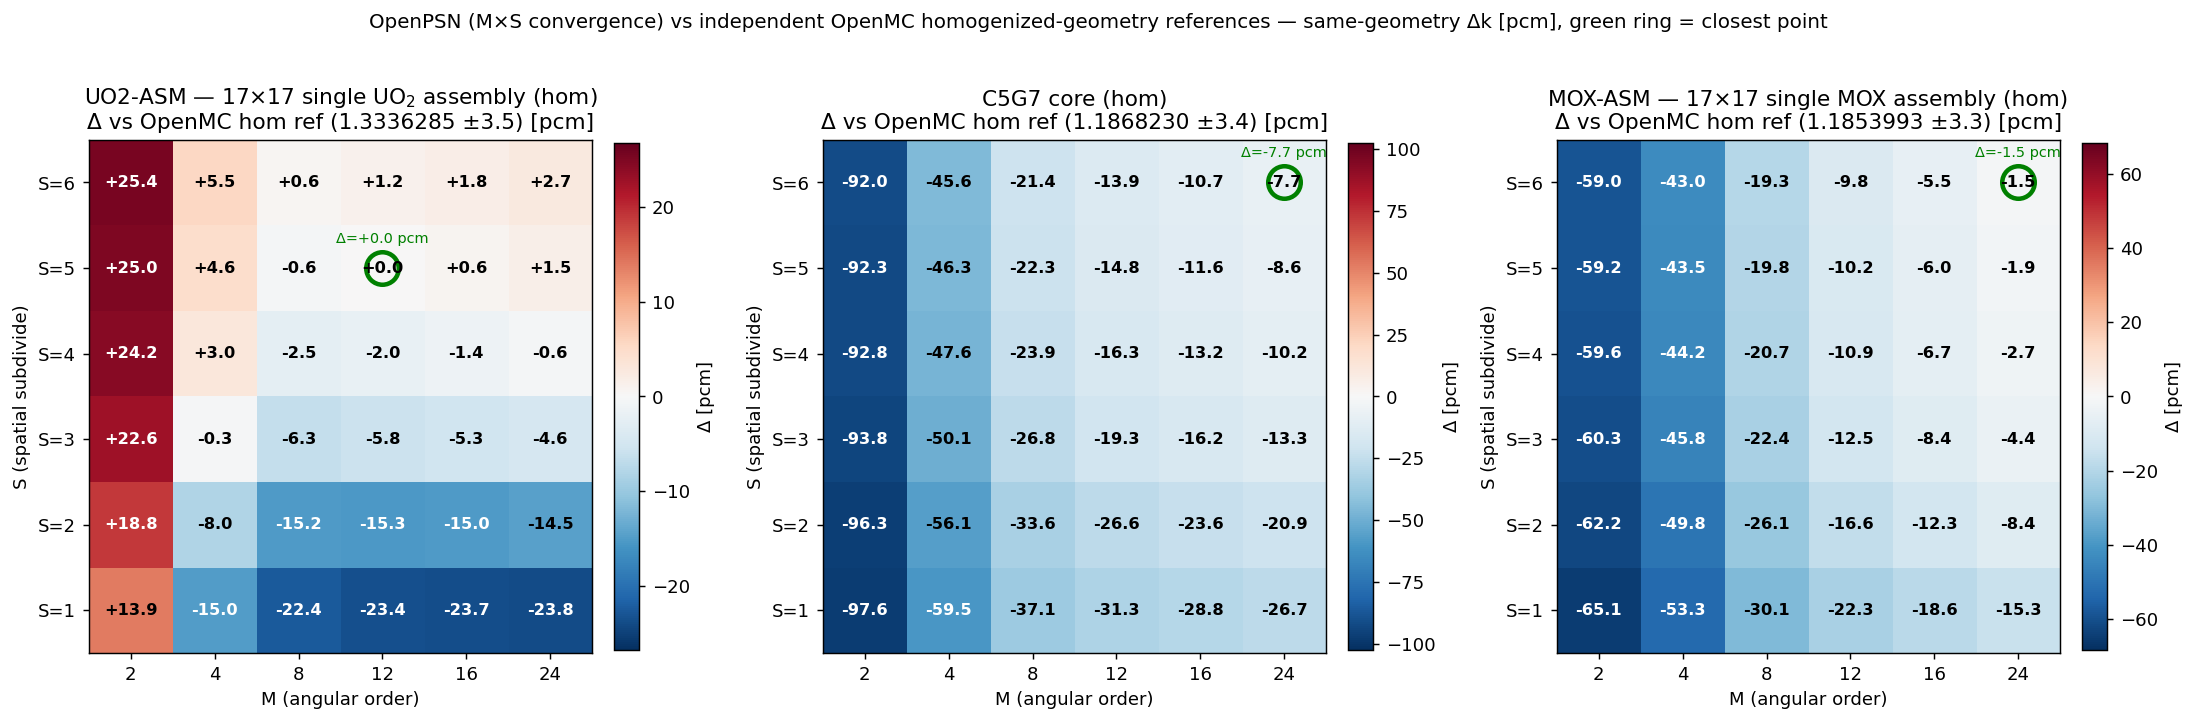
\includegraphics[width=0.98\textwidth]{c5g7_bww_sweep_heatmap.png}
\caption{Pinwise-homogenised (BWW) OpenPSN $\Delta\keff$ in pcm versus
the OpenMC homogenised reference, as a function of angular order $M$
(horizontal) and spatial sub-division $S$ (vertical). Left: single UO$_2$
assembly (ref.\ $1.3336285$); centre: C5G7-2D 1/4 core (ref.\
$1.1868230$); right: single MOX assembly (ref.\ $1.1853993$). All 36
points per panel; green ring = minimum-|$\Delta$| point of each panel.}
\label{fig:bww}
\end{figure}

\paragraph{Flux distribution at the best points.}
The best point of each geometry is not a sum of compensating local
errors: Figure~\ref{fig:bwwbest} compares its pin-averaged fission
source $\nu\Sigma_f\phi$ against the OpenMC homogenised-geometry
reference on the same BWW cross sections (the two sides differ only in
the transport method; the OpenMC field is the converged 7-group flux
contracted with the homogenised $\nu\Sigma_f$ --- the BWW library's
fission cross-section slot carries absorption, so the true fission
source is reconstructed from the flux, identically on both assemblies
and the core --- making both maps the same quantity, each normalised to
the unit fuel sum). On fuel pins the pin-by-pin relative error is
$0.03\%$ RMS (max $0.08\%$) on the UO$_2$ assembly, $0.04\%$ RMS
(max $0.10\%$) on the MOX assembly and $0.07\%$ RMS (max $0.25\%$) over
all $1056$ fuel pins of the 1/4 core. The best points therefore sit where
the local physics says they should: smooth, method-level biases, not
cancellations.

\begin{figure}[H]
\centering
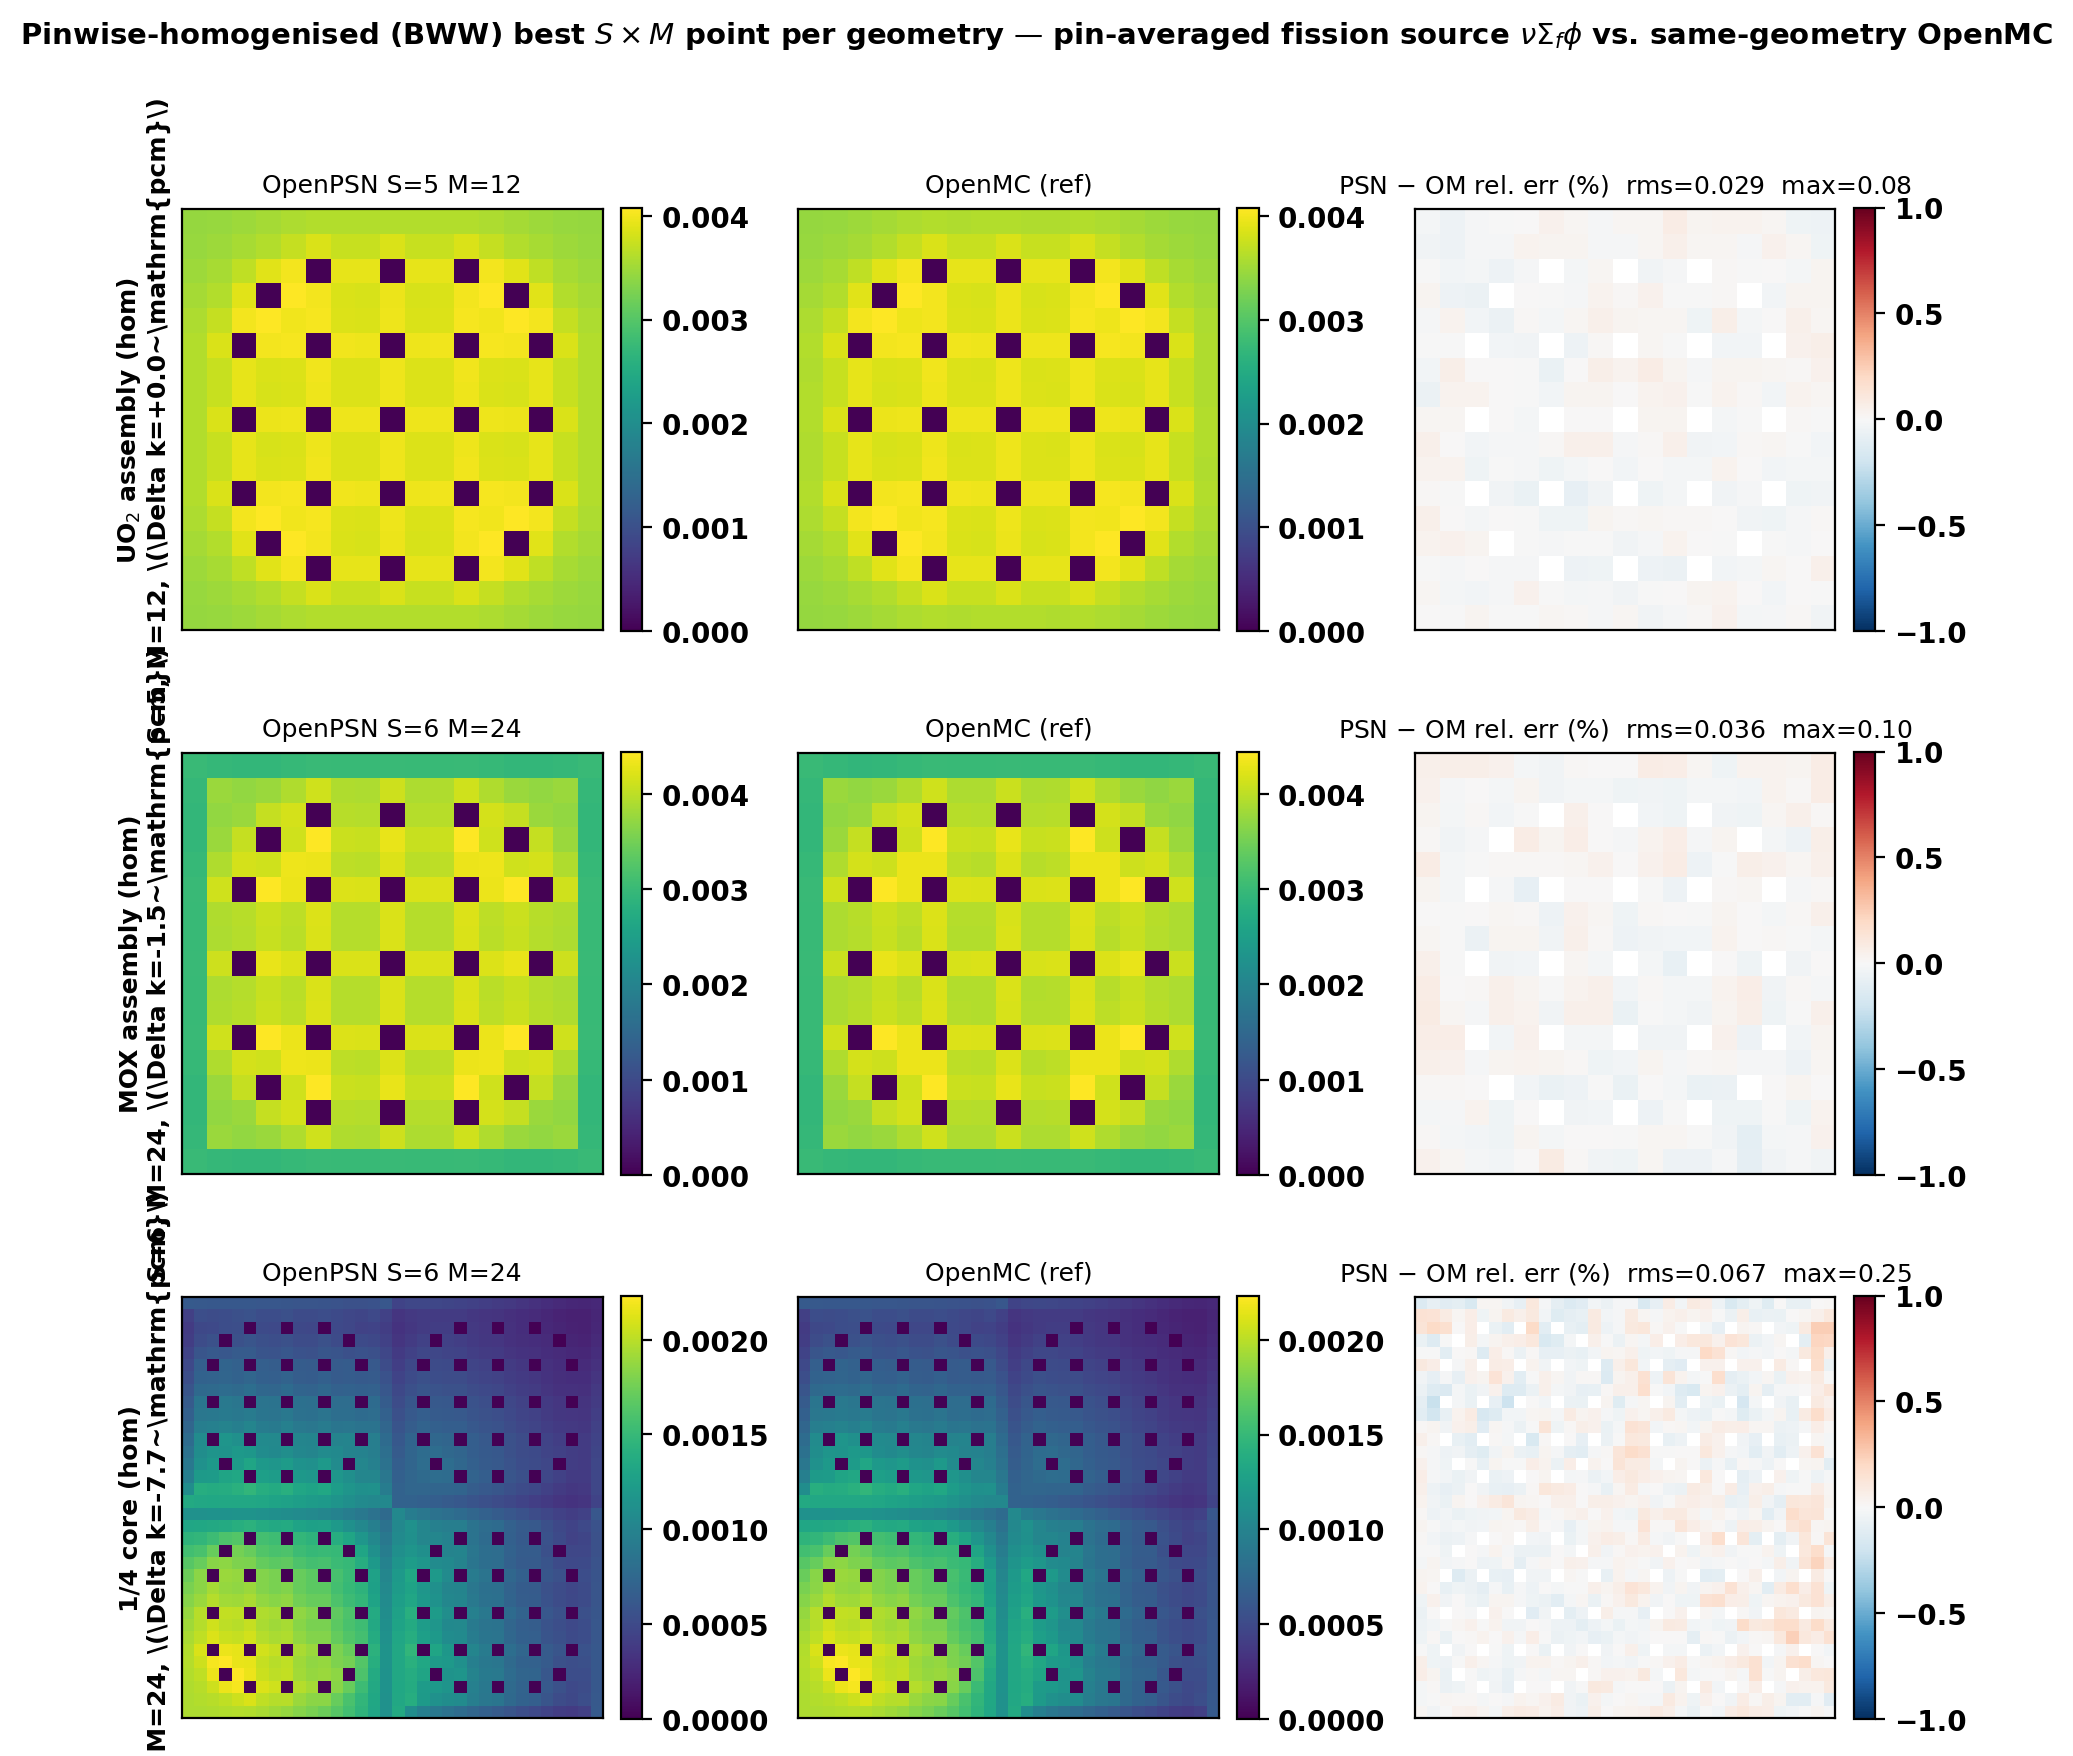
\includegraphics[width=0.98\textwidth]{c5g7_bww_best_fission.png}
\caption{Pinwise-homogenised (BWW) best $S\times M$ point per geometry
--- top: UO$_2$ assembly, $S{=}5,M{=}12$, $\Delta k=+0.0$~pcm; middle:
MOX assembly, $S{=}6,M{=}24$, $\Delta k=-1.5$~pcm; bottom: 1/4 core,
$S{=}6,M{=}24$, $\Delta k=-7.7$~pcm, cropped to the $2\times2$ fuel block
(the outer reflector-water region is omitted): pin-averaged fission source
$\nu\Sigma_f\phi$, OpenPSN (left), OpenMC same-geometry reference
(centre), pin-by-pin relative error on fuel pins (right; both maps
fuel-normalised).}
\label{fig:bwwbest}
\end{figure}

\subsection{Study II --- the rectangular-node model with explicit
intra-node structure}

\paragraph{Motivation and layout.}
Study I isolates the discretisation error of the nodal PSN model, but its
eigenvalue is still anchored to whatever homogenisation model feeds it. To
remove that model from the problem we use the rectangular-node extension
of Section~2.2: the circular C5G7 fuel rod ($r=0.54$~cm) is replaced by an
equal-area fuel square of side $s=\sqrt{\pi r^{2}}=0.95713$~cm centred on
the same 1.26~cm pitch, so that every pin cell becomes a $3\times3$ array
of rectangles (one fuel square plus eight water strips) and the whole core
is a globally edge-aligned rectangular tiling. Figure~\ref{fig:layout}
shows the layout. The pin pitch, the rod positions (including Gd pins,
which are the centre rectangle of their $3\times3$ block) and the total
fuel area are unchanged; the layout was verified node by node --- all
2601 fuel-centre rectangles of the 1/4 core coincide with the 2601 fuel
pins of the homogenised grid, and the total area reproduces
$4129.35~\mathrm{cm}^2$ exactly. Un-homogenised 7-group
cross sections (fuel, water, Gd, MOX) are then assigned directly to the
rectangles. Two discretisation knobs are now open: the angular order $M$
and the uniform spatial subdivision $S$ (Section~2.2), and we sweep both.

\begin{figure}[H]
\centering
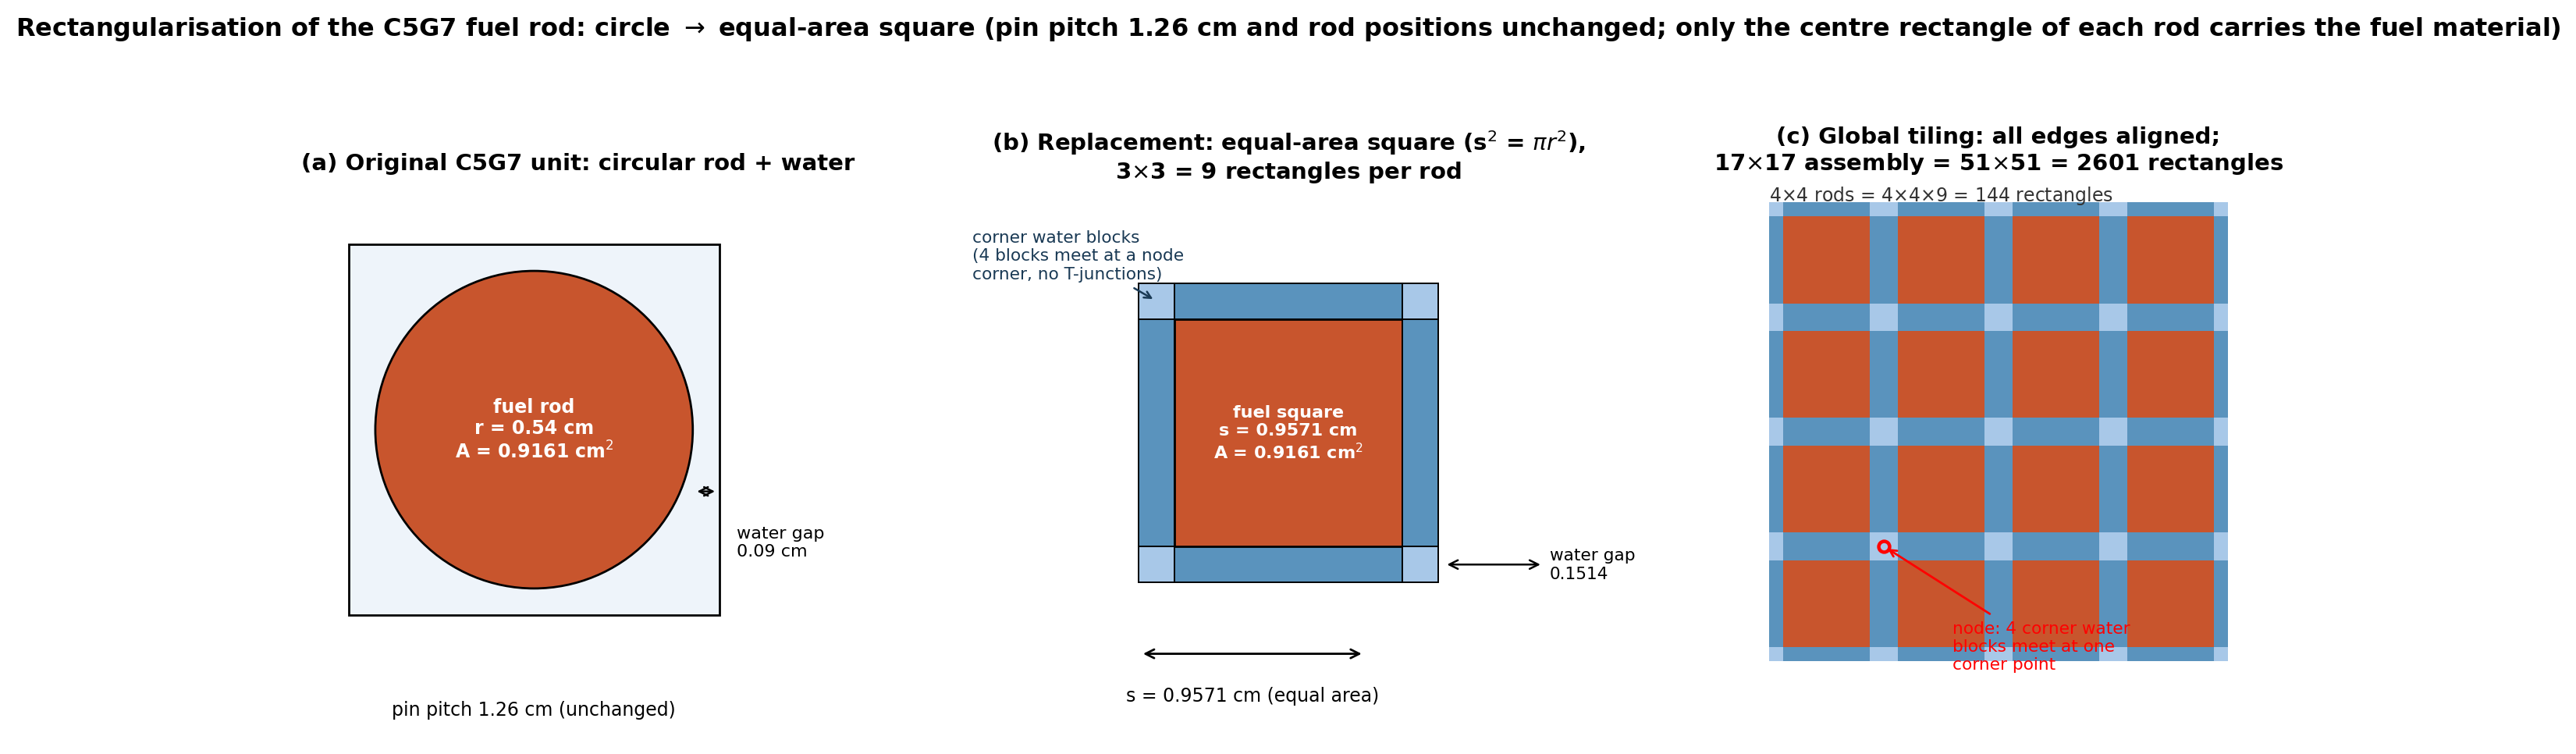
\includegraphics[width=0.98\textwidth]{c5g7_rect_layout.png}
\caption{Rectangularisation of the C5G7 pin cell. (a) Original circular
rod in its pitch cell (water gap 0.09~cm). (b) Equal-area fuel square
($s=0.95713$~cm, $s^2=\pi r^2$) with the pin cell split into $3\times3$
rectangles; the four corner water blocks of neighbouring pins meet at a
single node corner, so the tiling has no T-junctions. (c) Global tiling:
a $17\times17$ assembly is $51\times51=2601$ rectangles and the 1/4 core
is $153\times153=23409$.}
\label{fig:layout}
\end{figure}

\paragraph{$S\times M$ convergence of the $3\times3$ tiling.}
Table~\ref{tab:rectsm} and Figure~\ref{fig:rectsm} give the full
$S\times M$ sweep (UO$_2$/MOX assemblies: $S{=}1\ldots6$; 1/4 core:
$S{=}1,2$, the $S{=}3$ core grid being $9\times$ larger in node count and
only covered to $M{=}8$; un-homogenised material XS, every point
converged to
$10^{-10}$ in $|\Delta\keff|$) against the directly computed OpenMC run
on the \emph{identical} rectangular-rod geometry (Section~\ref{sec:rectref},
100k particles $\times$ 20200 batches, collision estimator, fixed seed):
the single UO$_2$ assembly ($51\times51$ rect.\ nodes, all edges
reflective, ref.\ $k=1.3347260$), the MOX assembly (same size, ref.\
$k=1.1851053$), and the 1/4 core ($153\times153$ rect.\ nodes, reflective
on the symmetry edges, vacuum on the open edges, ref.\ $k=1.1872176$).

\begin{table}[h]
\centering
\caption{Rectangular-node OpenPSN, $3\times3$ pin tiling: UO$_2$/MOX
assemblies at $S{=}1\ldots6$, 1/4 core at $S{=}1,2$ (at $S{=}3$ the core
grid grows $9\times$, only $M{=}2,4,8$ were computed). $\Delta k$ in pcm
versus the same-geometry pure-XS OpenMC reference (UO$_2$ assembly
$1.3347260$, MOX assembly $1.1851053$, 1/4 core $1.1872176$). Green
marker in Figure~\ref{fig:rectsm} = smallest $|\Delta k|$.}
\label{tab:rectsm}
\small
\begin{tabular}{l|rrrrrr}
\toprule
 & $M{=}2$ & $M{=}4$ & $M{=}8$ & $M{=}12$ & $M{=}16$ & $M{=}24$ \\
\midrule
\multicolumn{7}{l}{\emph{UO$_2$ assembly}}\\
$S{=}1$ & $+106.6$ & $-43.9$ & $-101.0$ & $-69.3$ & $-37.2$ & $+1.2$ \\
$S{=}2$ & $+93.1$ & $-71.7$ & $-132.6$ & $-99.3$ & $-66.9$ & $-28.1$ \\
$S{=}3$ & $+90.2$ & $-74.0$ & $-136.9$ & $-108.4$ & $-80.2$ & $-45.2$ \\
$S{=}4$ & $+89.2$ & $-74.3$ & $-138.4$ & $-111.2$ & $-85.8$ & $-51.9$ \\
$S{=}5$ & $+89.0$ & $-74.1$ & $-138.8$ & $-111.9$ & $-88.0$ & $-55.0$ \\
$S{=}6$ & $+88.9$ & $-74.1$ & $-139.0$ & $-112.6$ & $-89.0$ & $-56.5$ \\
\midrule
\multicolumn{7}{l}{\emph{MOX assembly}}\\
$S{=}1$ & $-893.6$ & $-769.8$ & $-503.5$ & $-319.0$ & $-207.9$ & $-98.9$ \\
$S{=}2$ & $-885.5$ & $-754.9$ & $-464.9$ & $-265.5$ & $-148.3$ & $-33.5$ \\
$S{=}3$ & $-889.5$ & $-760.7$ & $-488.3$ & $-304.3$ & $-198.3$ & $-92.2$ \\
$S{=}4$ & $-891.2$ & $-762.8$ & $-498.0$ & $-316.9$ & $-216.8$ & $-111.2$ \\
$S{=}5$ & $-891.9$ & $-763.9$ & $-502.6$ & $-322.9$ & $-226.0$ & $-122.4$ \\
$S{=}6$ & $-892.3$ & $-764.6$ & $-505.1$ & $-327.4$ & $-231.0$ & $-128.4$ \\
\midrule
\multicolumn{7}{l}{\emph{1/4 core}}\\
$S{=}1$ & $-254.3$ & $-246.6$ & $-184.3$ & $-110.9$ & $-61.1$ & $-10.2$ \\
$S{=}2$ & $-269.5$ & $-266.7$ & $-201.0$ & $-122.7$ & $-71.3$ & $-18.8$ \\
\bottomrule
\end{tabular}
\end{table}

\begin{figure}[H]
\centering
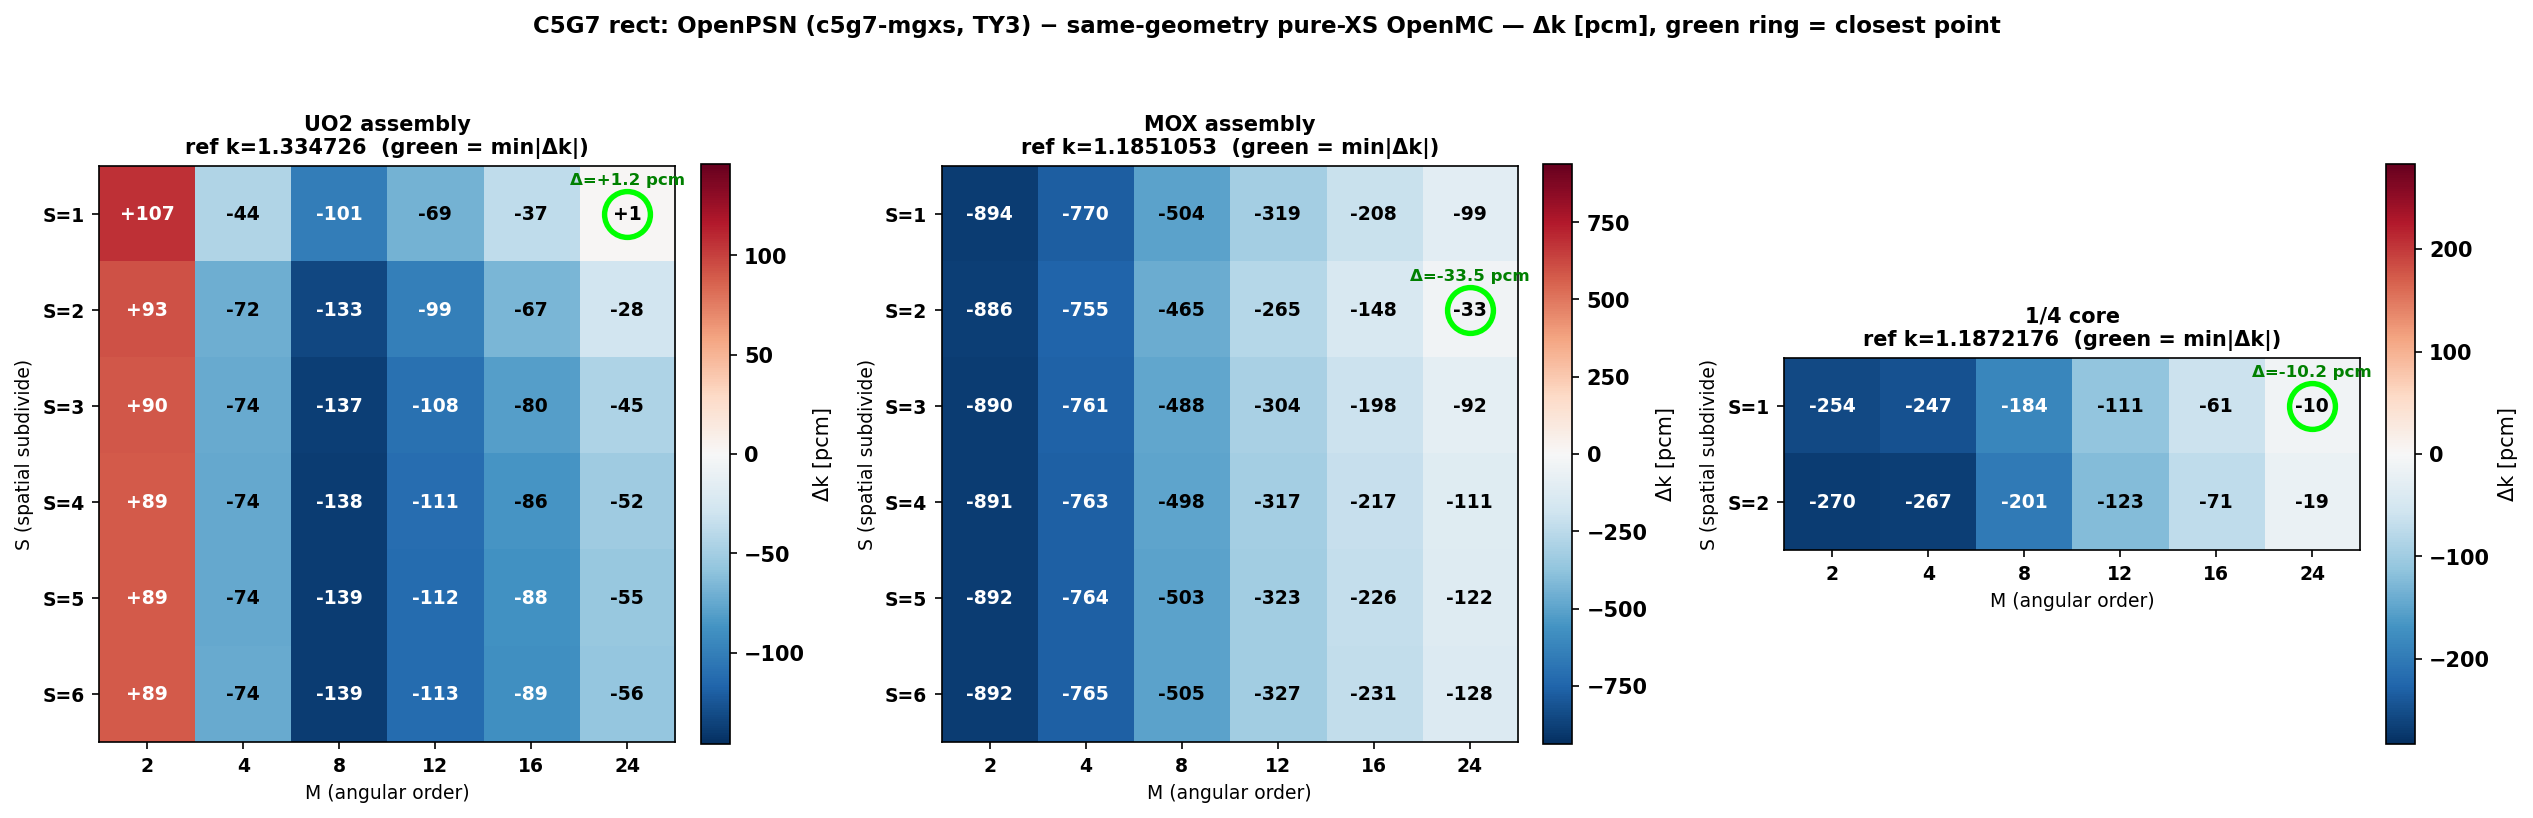
\includegraphics[width=0.98\textwidth]{rect_b4_sm_heatmap.png}
\caption{Same data as Table~\ref{tab:rectsm}, $\Delta k$ in pcm versus the
same-geometry pure-XS OpenMC reference; colour bars symmetric about zero,
green ring = point of smallest $|\Delta k|$ (UO$_2$: $S{=}1,M{=}24$,
$+1.2$~pcm; MOX: $S{=}2,M{=}24$, $-33.5$~pcm; core: $S{=}1,M{=}24$,
$-10.2$~pcm).}
\label{fig:rectsm}
\end{figure}

Figure~\ref{fig:rect33best} shows the fission field at the best
available configuration per geometry (Table~\ref{tab:rectsm}): the
UO$_2$ and core rows agree with OpenMC at the sub-percent level, while
the MOX row --- at its best subdivision $S{=}2$, still
$-33.5$~pcm off in $\keff$ --- carries that eigenvalue bias as a
spatially structured field-level deviation.

\begin{figure}[H]
\centering
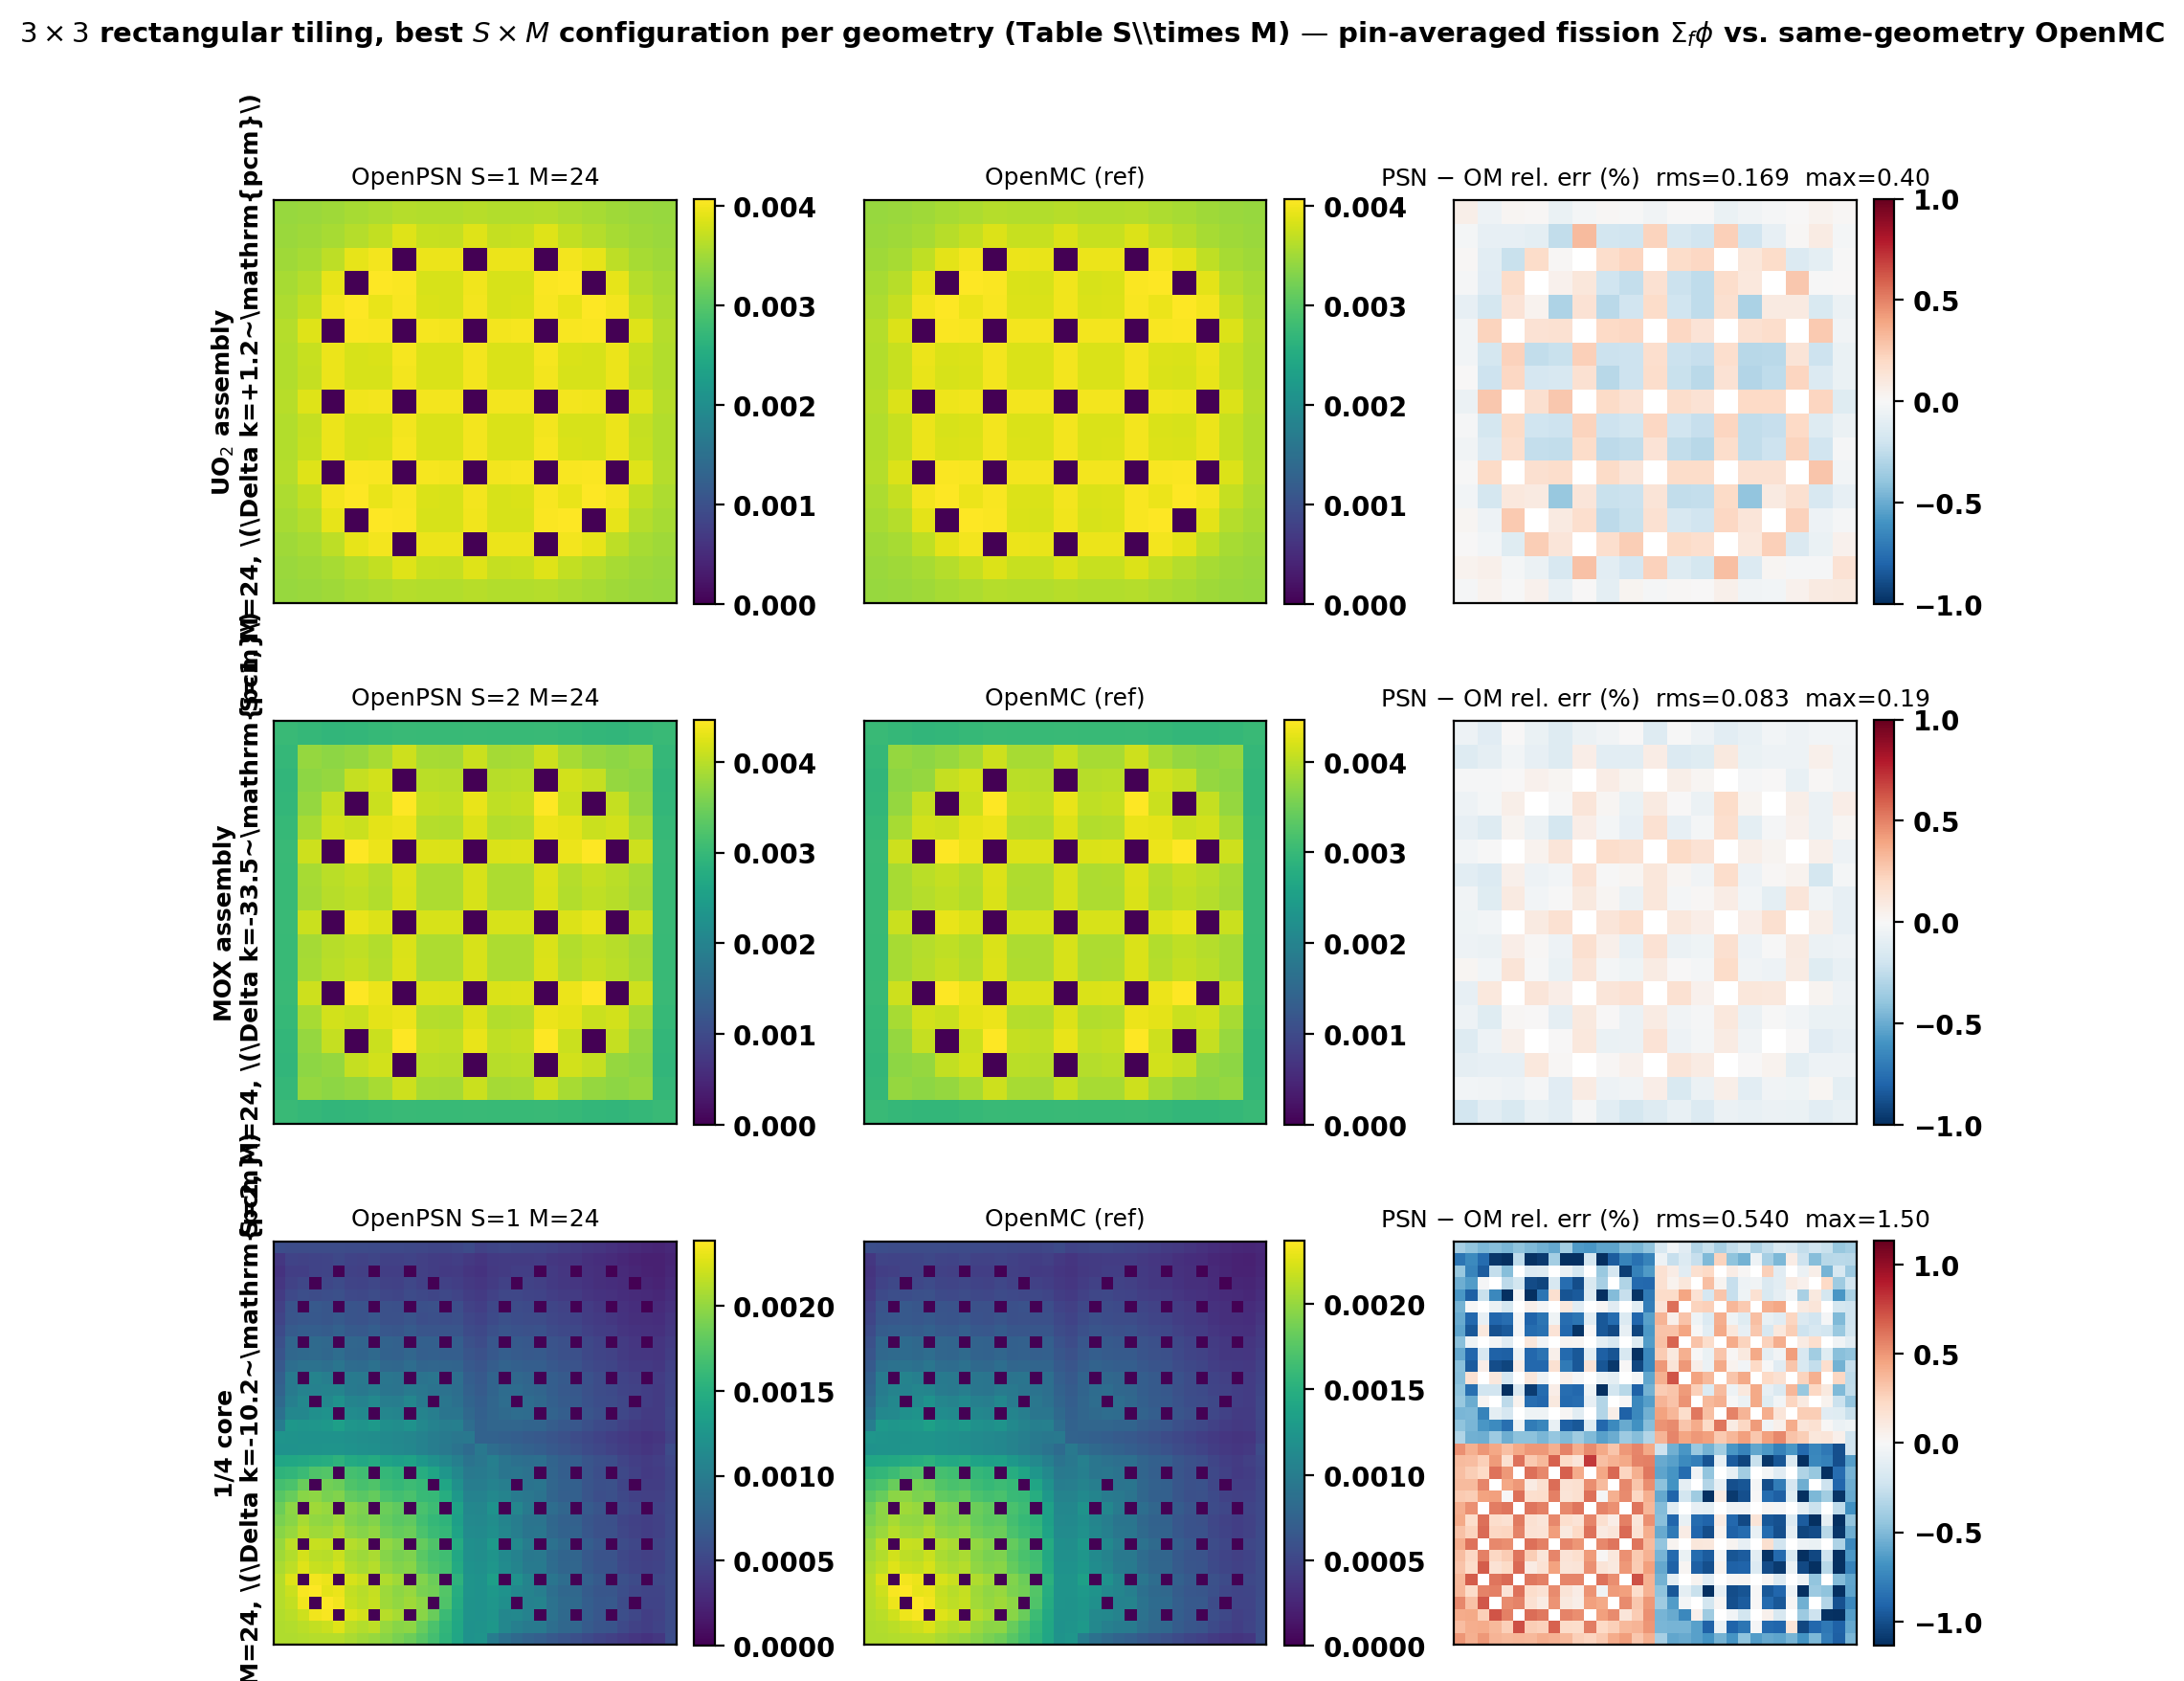
\includegraphics[width=0.71\textwidth]{c5g7_rect33_best_fission.png}
\caption{$3\times3$ rectangular tiling, best $S\times M$ configuration
per geometry (Table~\ref{tab:rectsm}): pin-averaged fission
$\Sigma_f\phi$, OpenPSN (left), OpenMC on the identical rectangular-rod
geometry (centre), pin-by-pin relative error on fuel pins (right; both
maps normalised to unit sum). Top: UO$_2$ assembly, $S{=}1,M{=}24$,
$\Delta k=+1.2$~pcm; middle: MOX assembly, $S{=}2,M{=}24$,
$\Delta k=-33.5$~pcm; bottom: 1/4 core, $S{=}1,M{=}24$,
$\Delta k=-10.2$~pcm (fuel region).}
\label{fig:rect33best}
\end{figure}

The sweep shows three things. (i)~On the UO$_2$ assembly the best point
($S{=}1,M{=}24$, $+1.2$~pcm) lies within the OpenMC standard error
($\pm3.6$~pcm): with a low-absorption fuel the nodal model is essentially
reference-grade on this geometry, and every deeper subdivision is worse,
monotonically from $-28.1$~pcm at $S{=}2$ to $-56.5$~pcm at $S{=}6$ ---
spatial subdivision is neutral-to-harmful.
(ii)~On the MOX assembly the tiling as constructed ($S{=}1$) is badly off
even at $M{=}24$ ($-98.9$~pcm); a single subdivision to $S{=}2$ improves it
to its best point ($-33.5$~pcm), and any further subdivision
($S{=}3\ldots6$) degrades it again, back to $-128.4$~pcm --- the
non-monotonic $S$-response with a single interior optimum at $S{=}2$ is
the clearest signature of the gap-node problem below. (iii)~On all three
geometries the $M$-convergence is non-monotonic at low order (an $M{=}8$
dip of $-101\ldots-504$~pcm) and only flattens out at $M{=}24$; on the
core the best point is $S{=}1,M{=}24$ ($-10.2$~pcm), again with $S{=}2$
slightly worse.

\paragraph{The slender water gap.}
The $S$-saturation pattern above points to a geometric cause. In the
$3\times3$ tiling the water-gap nodes are intrinsically slender: each edge
strip node measures $s/3 \times w = 0.3190\times0.1514$~cm, an aspect
ratio of $2.1{:}1$ (the corner nodes, $w\times w$, are square but carry
little physics). The uniform $S$ subdivision divides \emph{both}
dimensions by $S$, so every sub-node inherits the parent's aspect ratio ---
increasing $S$ refines the slender nodes but never makes them less
slender. The residual eigenvalue bias of Table~\ref{tab:rectsm} is
therefore plausibly anchored in the strip nodes, in a part of the mesh
that $S$-subdivision structurally cannot repair; this is consistent with
the UO$_2$ rows that degrade smoothly and monotonically as $S$ grows at
fixed $M$ (weak water coupling: subdivision adds nodes but never
re-shapes the strips), the MOX rows whose only relief is a single
subdivision --- best $S{=}2$, degrading again for $S{\ge}3$ (strong
fuel--water coupling in the gap) --- and the 1/4 core, whose $S{=}2$ row
is uniformly worse than $S{=}1$ across all $M$. The remedy is a tiling in which the water-gap nodes
are themselves close to square --- obtained by a finer, quasi-square fuel
split rather than by $S$. We first isolate this effect on a single pin.

\paragraph{Single-pin validation on the quasi-square ($6\times6$) split.}
As a controlled experiment we take the single UO$_2$ pin cell of the same
rectangularised layout and split the equal-area fuel square $6\times6$
instead of $3\times3$, giving an $8\times8$ base grid per pin cell
($6\times6$ fuel sub-nodes of side $s/6=0.15952$~cm plus water strips of
$0.15952\!\times\!0.15144$~cm, aspect ratio $1.05{:}1$ --- every node of the
cell is now close to square\textbf{, as illustrated in
Figure~\ref{fig:pin6split}}). The single cell with all-reflective
boundaries is converged to $10^{-10}$ in $|\Delta\keff|$ on a
$S\times M$ sweep of 60 points ($S=1\ldots6$, $M=2\ldots192$), against an
independently computed OpenMC reference on the same $8\times8$ geometry
(4000 batches, $k=1.3267918\pm8.2$~pcm). Table~\ref{tab:pin6} and
Figure~\ref{fig:pin6} summarise the sweep.

\begin{figure}[H]
\centering
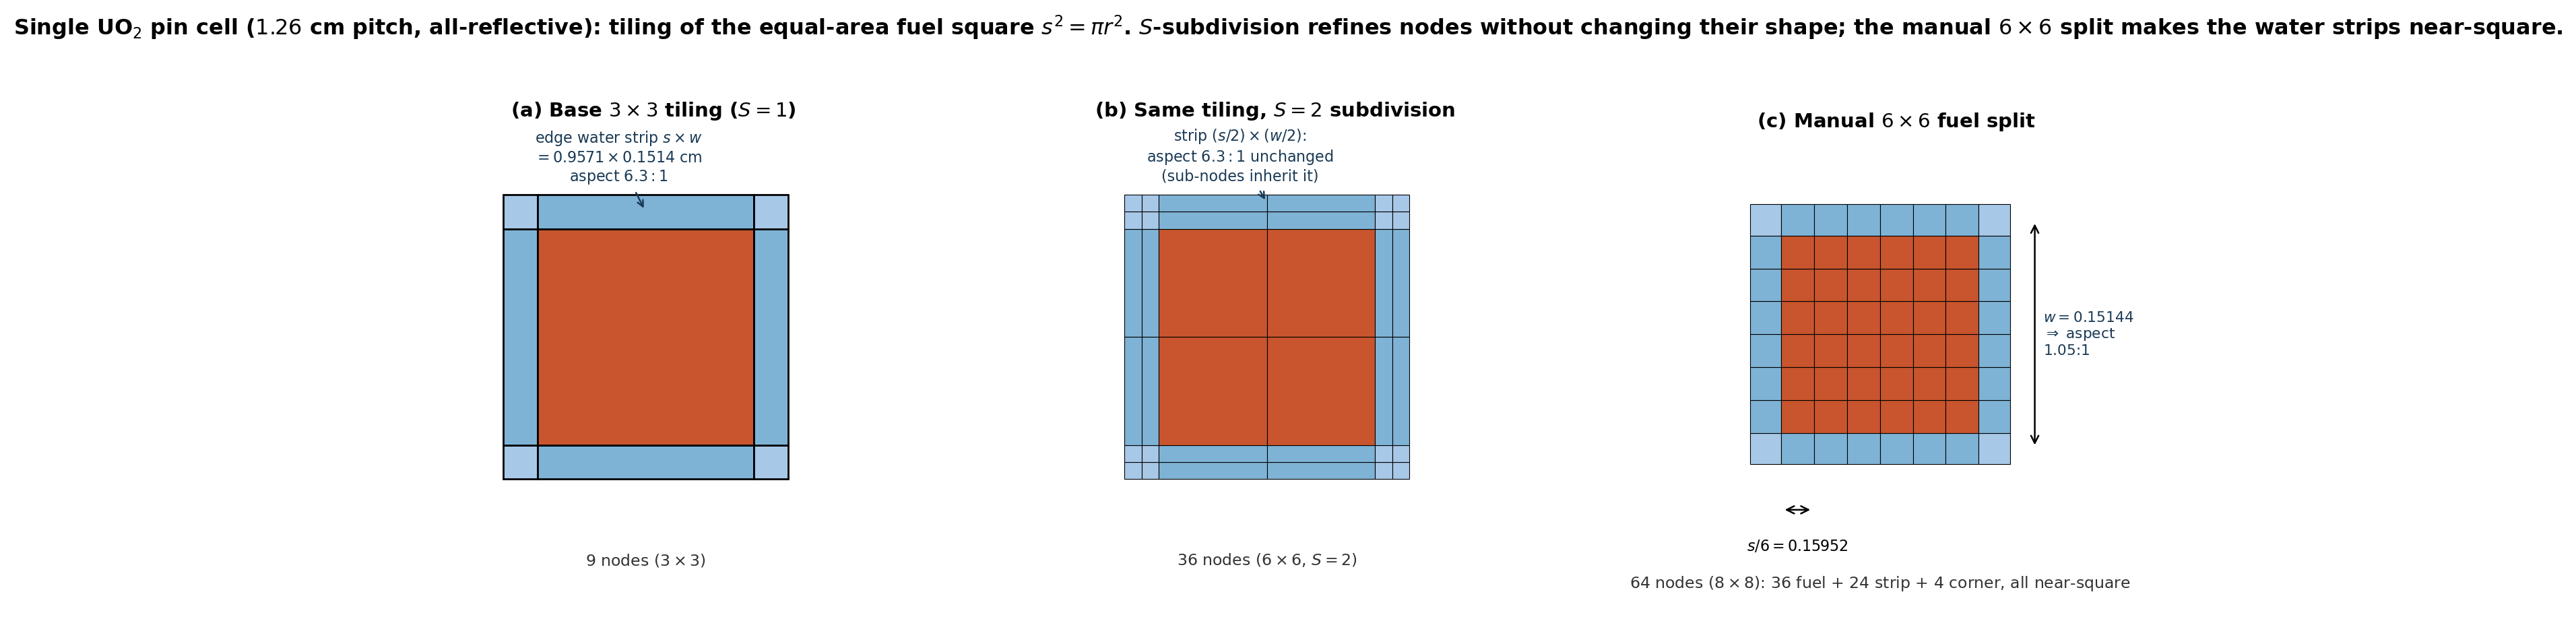
\includegraphics[width=0.98\textwidth]{pin6_manual_split.png}
\caption{Single UO$_2$ pin cell ($1.26$~cm pitch, all-reflective): tiling of
the equal-area fuel square $s^2=\pi r^2$. (a) Base $3\times3$ tiling: edge
water strips $s\times w = 0.9571\times0.1514$~cm (aspect $6.3{:}1$).
(b) The same tiling with $S{=}2$ subdivision: $36$ nodes, strips
$(s/2)\times(w/2)$, aspect unchanged --- $S$ refines but never reshapes the
nodes. (c) Manual $6\times6$ fuel split: $8\times8$ base grid
($64$ nodes), strips $s/6\times w = 0.15952\times0.15144$~cm, aspect
$1.05{:}1$; every node is now close to square.}
\label{fig:pin6split}
\end{figure}

\begin{table}[h]
\centering
\caption{Single UO$_2$ pin cell, $6\times6$ fuel split ($8\times8$ base
grid, all-reflective): $\Delta k$ in pcm versus the OpenMC reference
$1.3267918\pm8.2$. Green ring = best point $M{=}192$, $S{=}6$
($-8.7$~pcm, inside the reference's own standard error).}
\label{tab:pin6}
\small
\begin{tabular}{l|rrrrrrrrrr}
\toprule
 & $M{=}2$ & $M{=}4$ & $M{=}8$ & $M{=}12$ & $M{=}16$ & $M{=}24$ & $M{=}48$ & $M{=}72$ & $M{=}96$ & $M{=}192$ \\
\midrule
$S{=}1$ & $-73.0$ & $-182.9$ & $-208.2$ & $-165.1$ & $-132.0$ & $-88.0$ & $-41.6$ & $-28.2$ & $-22.6$ & $-16.5$ \\
$S{=}2$ & $-72.9$ & $-178.1$ & $-197.7$ & $-154.5$ & $-119.7$ & $-78.6$ & $-36.3$ & $-23.0$ & $-17.3$ & $-10.7$ \\
$S{=}3$ & $-72.6$ & $-176.8$ & $-195.1$ & $-151.9$ & $-116.7$ & $-75.9$ & $-35.1$ & $-21.8$ & $-16.2$ & $-9.6$ \\
$S{=}4$ & $-72.5$ & $-176.3$ & $-193.9$ & $-150.8$ & $-115.4$ & $-74.7$ & $-34.3$ & $-21.1$ & $-15.7$ & $-9.1$ \\
$S{=}5$ & $-72.4$ & $-176.0$ & $-193.4$ & $-150.2$ & $-114.7$ & $-74.1$ & $-33.9$ & $-20.7$ & $-15.4$ & $-8.9$ \\
$S{=}6$ & $-72.4$ & $-175.8$ & $-193.0$ & $-149.9$ & $-114.3$ & $-73.7$ & $-33.6$ & $-20.5$ & $-15.2$ & $-8.7$ \\
\bottomrule
\end{tabular}
\end{table}

\begin{figure}[H]
\centering
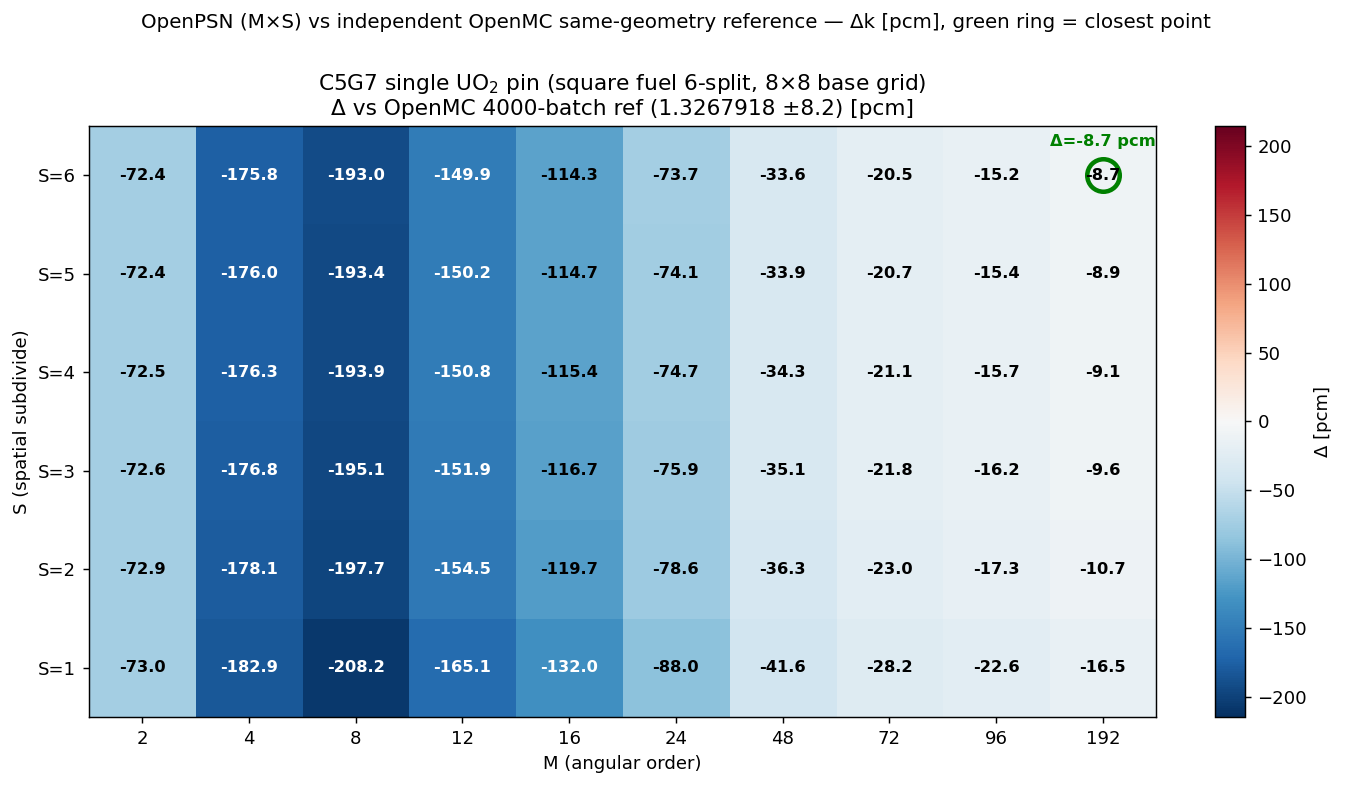
\includegraphics[width=0.98\textwidth]{pin6_sm.png}
\caption{Single-pin $6\times6$-split $S\times M$ sweep, $\Delta k$ in pcm
versus the OpenMC same-geometry reference; green ring = best point
($M{=}192$, $S{=}6$, $\Delta=-8.7$~pcm).}
\label{fig:pin6}
\end{figure}

On the quasi-square single pin the model converges to within the
reference's own Monte Carlo standard error ($-8.7$~pcm at $M{=}192$,
$S{=}6$) --- and the spatial field agrees even more tightly: at the best
configuration the node-level fission-rate map differs from OpenMC by
$0.05\%$ RMS (max $0.10\%$) and the scalar flux by $0.01\%$ RMS
(max $0.03\%$) over the fuel nodes (Figure~\ref{fig:pin6flux}). The
convergence is smooth in $M$ once the $M{=}8$ angular damped-oscillation
dip is passed, and $S$ contributes a further $\sim8$~pcm of improvement
from $S{=}1$ to $S{=}6$ that is still active at $M{=}192$ --- i.e.\ on a
quasi-square mesh both knobs are effective. This contrasts with the
$3\times3$ tiling, where the $S{=}1\to2$ change buys at most a factor of
three on the MOX bias and the best subdivision is geometry-dependent
(Table~\ref{tab:rectsm}).

\begin{figure}[H]
\centering
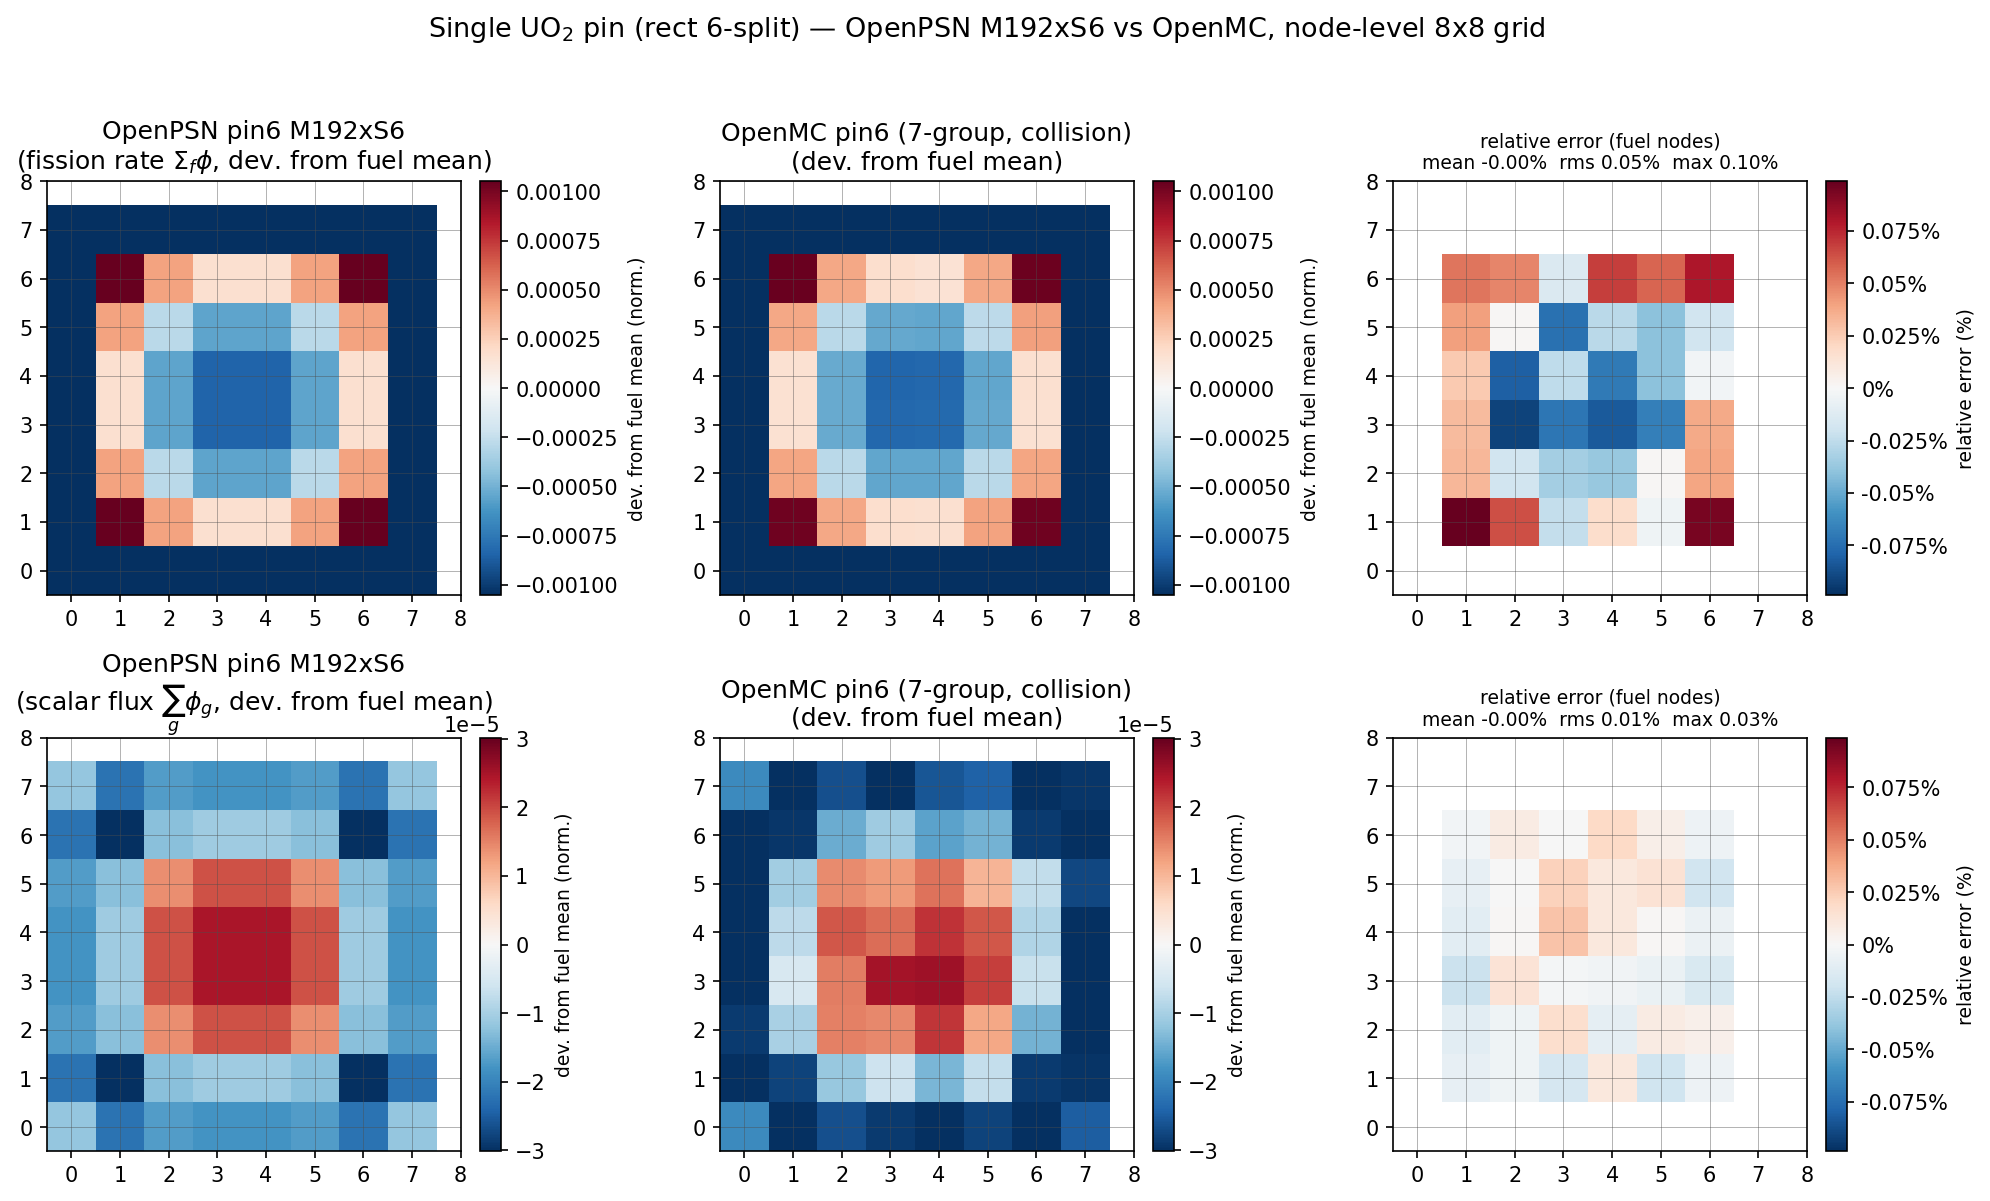
\includegraphics[width=0.98\textwidth]{pin6_flux_compare_M192S6.png}
\caption{Single-pin $6\times6$ split, best configuration ($M{=}192$,
$S{=}6$): node-level ($8\times8$) fission rate $\Sigma_f\phi$ (top) and
scalar flux $\sum_g\phi_g$ (bottom), OpenPSN vs.\ OpenMC (7-group,
collision estimator) with the pin-by-pin relative error on the fuel nodes;
deviation from the fuel-node mean, maps normalised to unit fuel sum.
Fission: mean $-0.00\%$, RMS $0.05\%$, max $0.10\%$; flux: RMS $0.01\%$,
max $0.03\%$.}
\label{fig:pin6flux}
\end{figure}

\paragraph{Quasi-square tiling of the full geometries.}
We now apply the single-pin quasi-square split to the full benchmark:
every fuel square of the $3\times3$ tiling is subdivided $6\times6$, so
each pin cell becomes an $8\times8$ block of rectangles --- fuel
sub-nodes $0.15952\times0.15952$~cm and water strips
$0.15952\times0.15144$~cm, aspect ratio $1.05{:}1$. The $17\times17$
assembly becomes $136\times136=18496$ rectangles and the 1/4 core
$408\times408=166464$; the pin-centre material layout, the rod positions,
the fuel area and the total area are unchanged (verified node by node,
max cell-width deviation $0.0$). Because the physical geometry is
identical to the rectangular-rod problem of Section~\ref{sec:rectref},
the \emph{existing} same-geometry OpenMC references
($1.3347260$, $1.1851053$, $1.1872176$) apply without re-running: the
comparison is again a pure method difference.

\paragraph{$M$-convergence of the quasi-square tiling.}
{\emergencystretch=1.5em\relax
Table~\ref{tab:rect6} and Figure~\ref{fig:rect6keff} give the $S{=}1$
sweep, $M=2\ldots96$ on the two assemblies (core $M{\ge}24$ and the
$M{=}192$ extension in progress). Two features stand out. First,
$M$-convergence is markedly faster than on the
$3\times3$ tiling at comparable resolution: on the MOX assembly the
bias drops from $-893.7$ to $+2.1$~pcm over $M{=}2\ldots96$, whereas
the $3\times3$ tiling reaches $-98.9$~pcm at $M{=}24$ ($-33.5$~pcm only
with $S{=}2$);
the low-order $M{=}8$ dip remains but is shallower on the core. Second,
the pin-averaged fission distribution converges \emph{far} ahead of the
eigenvalue: on both assemblies the pin-by-pin RMS error against OpenMC
is at or below $0.09\%$ from $M{=}8$ onward ($0.056\%$ UO$_2$ and
$0.069\%$ MOX at $M{=}96$), while $\Delta k$ still carries
$-161\ldots-28.7$~pcm of bias on UO$_2$ and $-512\ldots+2.1$~pcm on MOX
over the same range --- the intra-fuel quasi-square split
delivers the full spatial shape of the solution at a fraction of the
angular order needed for the global eigenvalue.}

\begin{table}[h]
\centering
\caption{Quasi-square ($6\times6$ fuel split) OpenPSN, $S{=}1$: $\Delta k$
in pcm versus the same-geometry pure-XS OpenMC reference (refs.\ as in
Table~\ref{tab:rectsm}). Dombey two-point source extrapolation on
MOX/core. Core $M{\ge}24$ and the $M{=}192$ extension pending.}
\label{tab:rect6}
\small
\begin{tabular}{l|rrrrrrrr}
\toprule
 & $M{=}2$ & $M{=}4$ & $M{=}8$ & $M{=}12$ & $M{=}16$ & $M{=}24$ & $M{=}48$ & $M{=}96$ \\
\midrule
\emph{UO$_2$ assembly} & $+86.2$ & $-85.6$ & $-160.7$ & $-138.4$ & $-115.7$ & $-82.6$ & $-44.9$ & $-28.7$ \\
\emph{MOX assembly} & $-893.7$ & $-768.5$ & $-511.6$ & $-333.2$ & $-235.8$ & $-129.2$ & $-33.2$ & $+2.1$ \\
\emph{1/4 core} & $-278.8$ & $-281.5$ & $-232.4$ & $-166.9$ & $-126.2$ & $\cdots$ & $\cdots$ & $\cdots$ \\
\bottomrule
\end{tabular}
\end{table}

\begin{figure}[H]
\centering
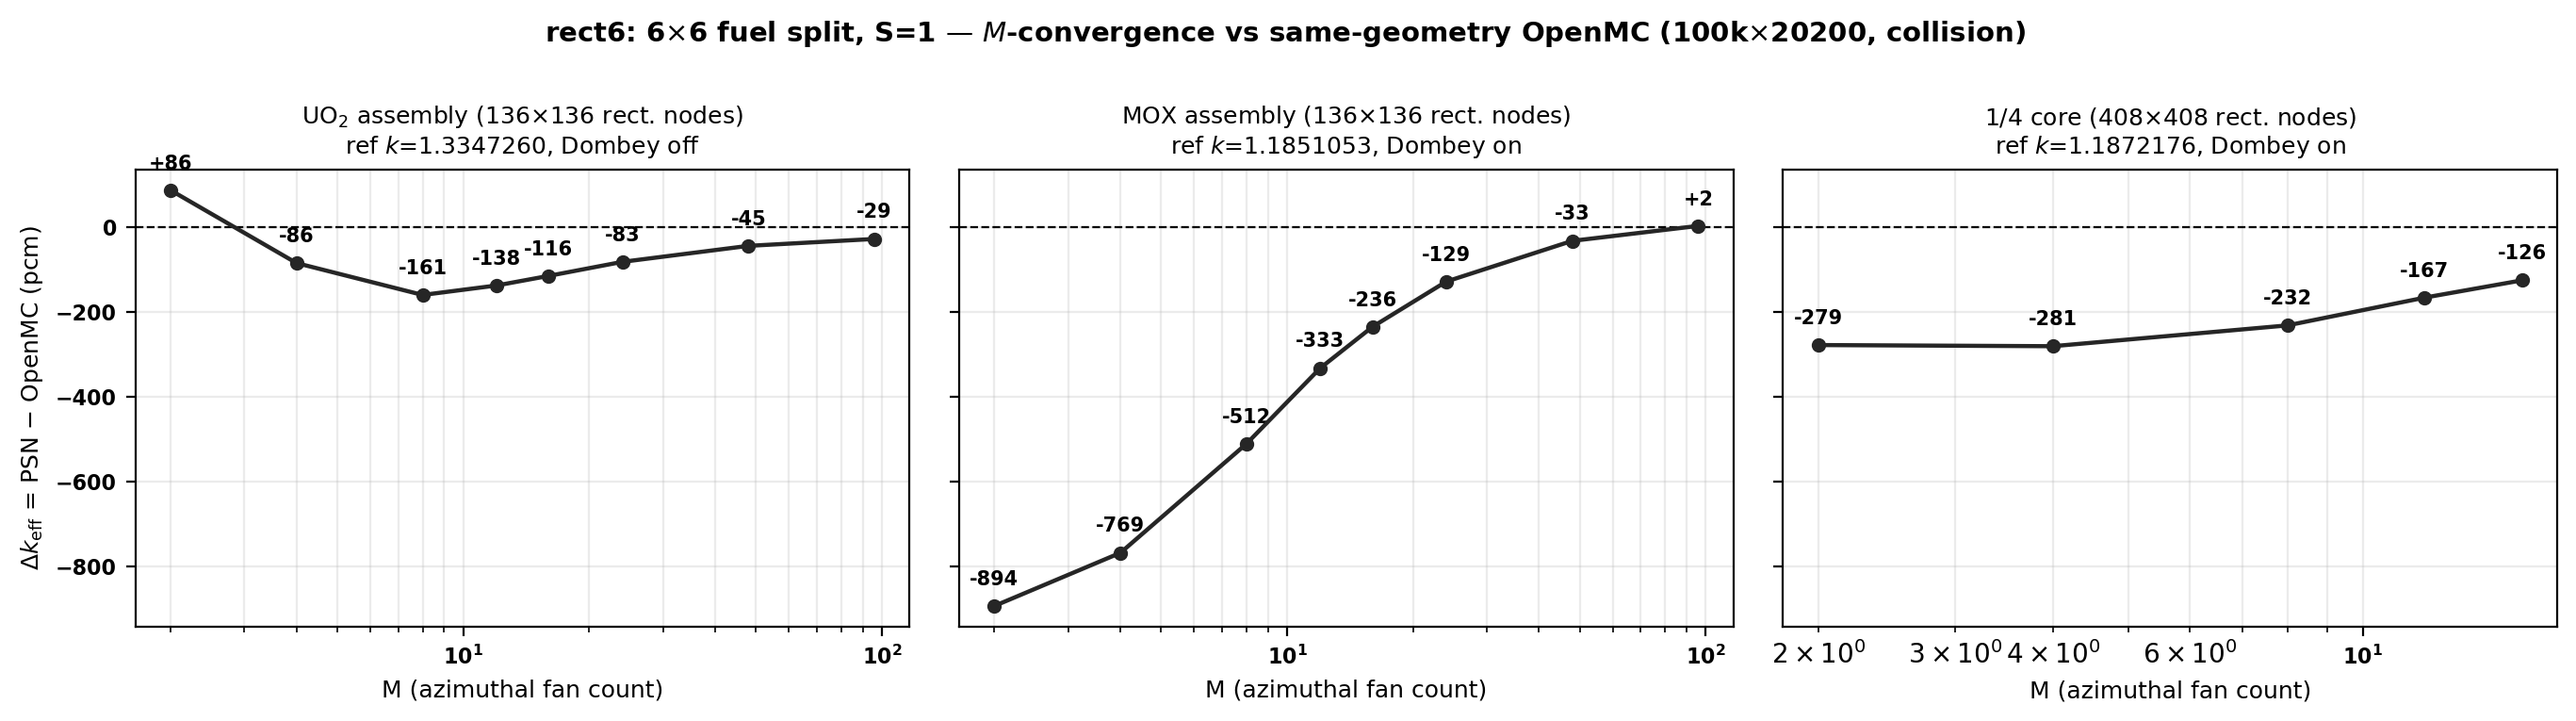
\includegraphics[width=0.98\textwidth]{rect6_keff_conv.png}
\caption{Quasi-square tiling, $S{=}1$: $\Delta k$ versus $M$ against the
same-geometry OpenMC reference (100k$\times$20200, collision estimator).
UO$_2$ assembly (left) shows the non-monotonic low-order behaviour; the
MOX assembly (centre) and 1/4 core (right) converge monotonically with
$M$.}
\label{fig:rect6keff}
\end{figure}

Figure~\ref{fig:rect6best} compares the pin-averaged fission maps
$\Sigma_f\phi$ of the best quasi-square configuration (smallest
$|\Delta k|$ per geometry, currently $M{=}96$ on both assemblies) against
the OpenMC reference on the identical geometry, using the same
$\nu$-correction and fuel-block normalisation as
Section~\ref{sec:rectref}. On the UO$_2$ assembly the pin-by-pin
difference is a mean of $+0.002\%$ and an RMS of $0.056\%$ (max
$0.19\%$, p95 $0.10\%$); on the MOX assembly a mean of $-0.006\%$ and an
RMS of $0.069\%$ (max $0.21\%$, p95 $0.12\%$) --- i.e.\ the intra-fuel
quasi-square tiling matches the reference pin power to well under one
tenths of a percent on both assemblies, with the residual confined to a
few corner pins.

\begin{figure}[H]
\centering
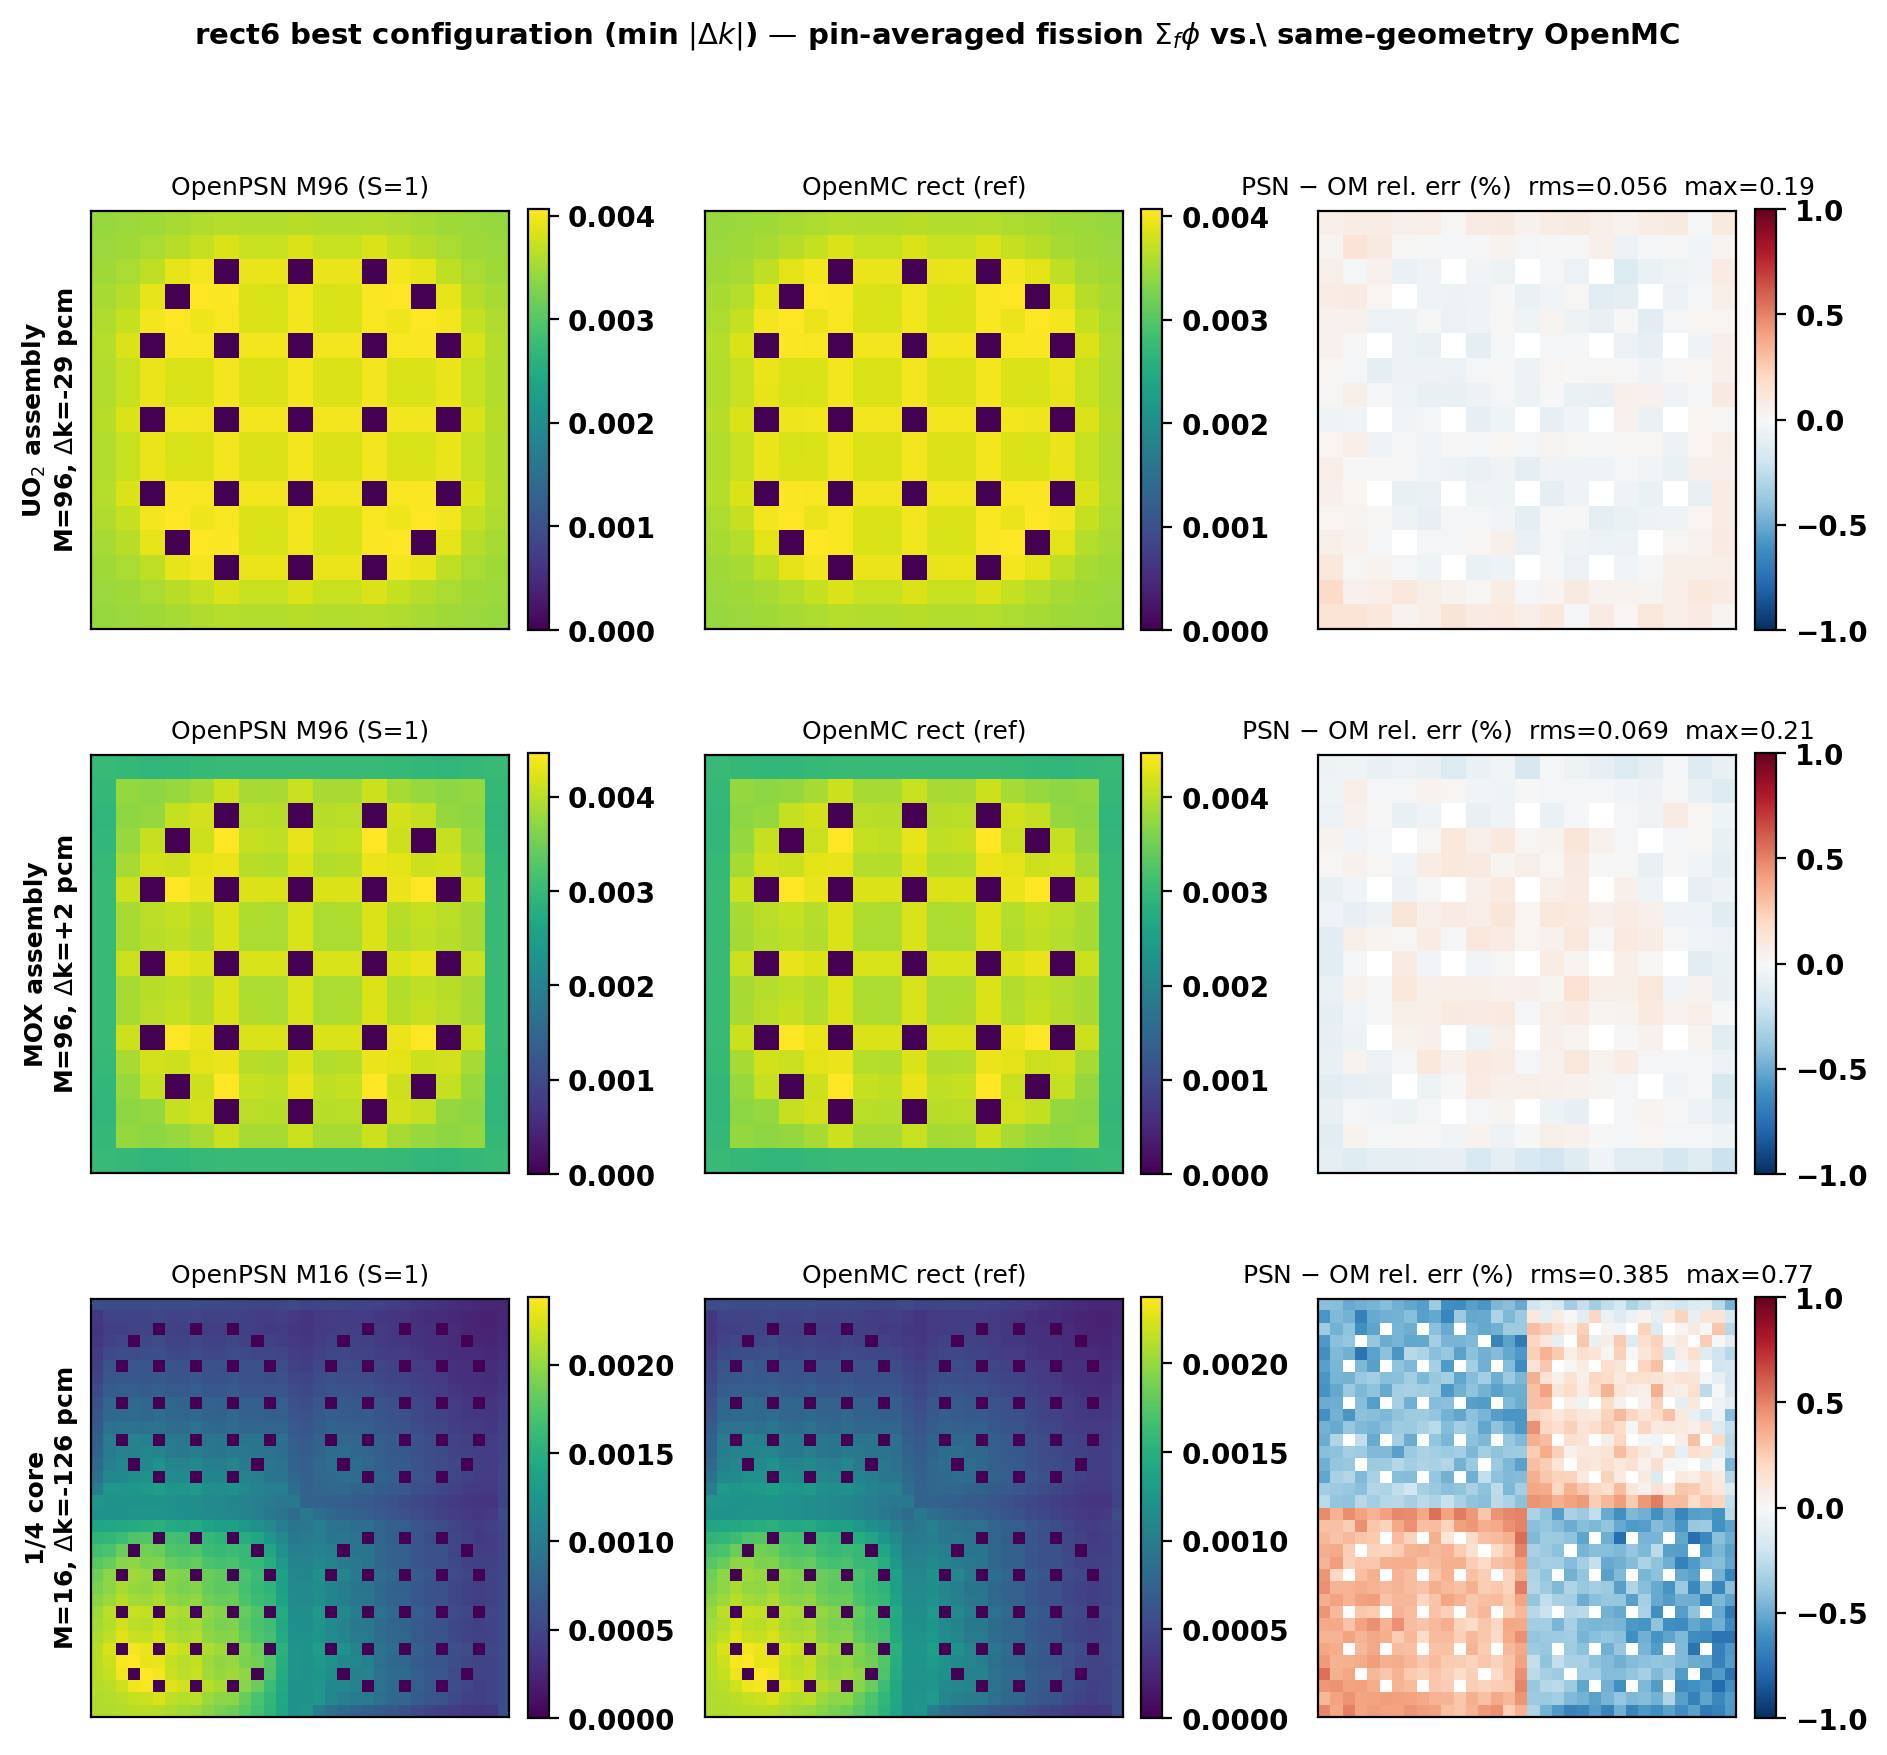
\includegraphics[width=0.98\textwidth]{rect6_best_fission.png}
\caption{Quasi-square tiling, best configuration per geometry (min
$|\Delta k|$, $S{=}1$): pin-averaged fission $\Sigma_f\phi$, OpenPSN
(left), OpenMC same-geometry reference (centre), pin-by-pin relative error
on fuel pins (right; both maps fuel-block normalised). Top: UO$_2$
assembly, $M{=}96$; middle: MOX assembly, $M{=}96$; bottom: 1/4 core
(interim best $M{=}16$, $M{\ge}24$ in progress), cropped to the
$2\times2$ fuel block --- the outer reflector-water region is omitted.}
\label{fig:rect6best}
\end{figure}

\label{sec:rectref}
\paragraph{Rectangular-rod reference.}
{\emergencystretch=1.5em\relax
The circular pin cell is the benchmark's reference geometry, while the PSN
nodes tile the same cell with an equal-area square fuel block (side
$0.9571$~cm, water gap $0.1514$~cm). To separate the geometric effect from
the method difference we run OpenMC on exactly that rectangular-rod geometry
(same un-homogenised data, same collision-estimator pin tallies, $20200$
batches $\times 10^{5}$ particles, fixed seed): the square-rod UO$_2$
assembly returns $\keff = 1.3347260$ ($\pm 3.6$~pcm), the MOX assembly
$1.1851053$ ($\pm 3.3$~pcm, identical clone of the UO$_2$ run with only the
pin material grid changed to the C5G7 MOX layout) and the 1/4 core
$1.1872176$ ($\pm 3.4$~pcm). Against these same-geometry references the
$3\times3$ tiling behaves as in Table~\ref{tab:rectsm} and
Figure~\ref{fig:rect33best}; the pin-level fission maps $\Sigma_f\phi$
of the $3\times3$ tiling at $S{=}1,M{=}24$ agree with OpenMC to
$0.17\%$ RMS (max $0.40\%$) on the UO$_2$ assembly and
$0.54\%$ RMS (max $1.50\%$) over all $1056$ fuel pins of
the 1/4 core, while the MOX assembly carries the $-98.9$~pcm eigenvalue
bias as a spatially structured field-level deviation; the quasi-square
tiling holds at or below $0.09\%$ RMS on both assemblies
from $M{\ge}8$ and settles at $0.06\text{--}0.07\%$ by $M{=}96$
(Figure~\ref{fig:rect6best}).}\

\clearpage
\subsection{Comparison with the published diffusion / SN / nodal landscape}
The original NEA report~\cite{nea2003} tabulates 20 deterministic codes on
C5G7-2D. Table~\ref{tab:lit} reproduces the diffusion- and nodal-family
values we could extract from it, together with recent P1/SP3/SN/nodal
literature results and our own OpenPSN result.

\begin{table}[h]
\centering
\caption{C5G7-2D $\keff$ by method class (2-D multi-group, homogenised pin
model unless noted). NEA-2003 $k$ values (its Table~17) plus recent P1/SP3
literature. $\Delta$ = $(k-1.18646)\times10^{5}$ in pcm, except where stated
(STELLA vs its PEACH reference 1.18716). The original NEA table prints the
relative per-cent error against its MCNP reference 1.18655; the pcm values
here are recomputed from the printed $k$ against 1.18646.}
\label{tab:lit}
\small
\begin{tabular}{llcc}
\toprule
method class & code & $\keff$ & $\Delta$ (pcm) \\
\midrule
\multicolumn{4}{l}{\emph{Pure P1 diffusion}}\\
diffusion (FEM) & CRONOS2 & 1.18323 & $-323$ \\
P1 (pin-hom) & STELLA-P1~\cite{stella2017} & 1.18426 & $-290$ (vs PEACH)\\
\midrule
\multicolumn{4}{l}{\emph{SN}}\\
SN-FEM & CRONOS2-SN & 1.18338 & $-308$ \\
SN-FDM & DORT-GRS & 1.18482 & $-164$ \\
SN-FDM & DORT-ORNL & 1.18496 & $-150$ \\
SN-FDM & TWODANT & 1.18668 & $+22$ \\
SN (diamond diff.) & PARTISN & 1.18637 & $-9$ \\
SN (unstructured) & PERICLES & 1.18658 & $+12$ \\
\midrule
\multicolumn{4}{l}{\emph{High-order nodal $P_n$ / surf.\ harmonics}}\\
$P_n$-nodal (FEM) & VARIANT-SE & 1.18495 & $-151$ \\
$P_n$-nodal + int.\ transp.\ & VARIANT-ISE & 1.18745 & $+99$ \\
surface harm.\ (G3/P2) & SUHAM-2D & 1.18628 & $-18$ \\
\midrule
\multicolumn{4}{l}{\emph{MOC}}\\
MOC & CHAPLET & 1.18656 & $+10$ \\
MOC & MCCG3D & 1.18657 & $+11$ \\
MOC & DeCART & 1.18660 & $+14$ \\
MOC & APOLLO2 & 1.18618 & $-28$ \\
MOC & CRX & 1.18813 & $+167$ \\
MOC (stoch.\ rays) & UNKGRO & 1.18523 & $-123$ \\
\midrule
\multicolumn{4}{l}{\emph{This work}}\\
\rowcolor{gray!15}
PSN nodal (rect.\ node, $M{=}16$) & OpenPSN & 1.1866067 & $+14.7$ \\
\bottomrule
\end{tabular}
\end{table}

\emph{Readings.}
\begin{itemize}
\item \textbf{Pure P1 diffusion is systematically low} --- CRONOS2
  $-323$~pcm ($-0.27\%$), STELLA-P1
  $-290$~pcm vs its PEACH MOC reference 1.18716: no transport correction and
  no self shielding.
\item \textbf{SN spans $-308$ (CRONOS2-SN) to $+22$~pcm (TWODANT);
  DORT $-164$/$-150$; the better-differenced / unstructured variants
  PARTISN ($-9$) and PERICLES ($+12$) within $\pm0.01\%$.}
\item \textbf{High-order nodal $P_n$ / surface harmonics} spans
  $-151$ (VARIANT-SE) to $+99$~pcm (VARIANT-ISE); SUHAM-2D $-18$; VARIANT-ISE
  also has the best pin power in the original table (MRE 0.11\%).
\item \textbf{MOC (explicit pin geometry) clusters within $\pm28$~pcm}
  (CHAPLET $+10$, MCCG3D $+11$, DeCART $+14$, APOLLO2 $-28$), with two
  outliers (CRX $+167$, UNKGRO $-123$); TWODANT is SN-FDM ($+22$); the
  high-fidelity Rattlesnake converged limit is $1.186446$
  ($\sim$\SI{1}{pcm} from the 1.186456 reference).
\item \textbf{OpenPSN in this work.} The two C5G7 studies of
  Sections~4.3--4.4 bound the answer from both sides. With the
  self-shielding-aware BWW pinwise homogenisation, the best points of the
  $S\times M$ sweep are $+0.0$~pcm (UO$_2$ assembly), $-1.5$~pcm (MOX
  assembly) and $-7.7$~pcm (1/4 core) vs.\ the OpenMC homogenised
  references --- the two assemblies inside their own Monte Carlo standard
  errors; with the
  rectangular-node model that removes homogenisation entirely, $M{=}16$
  lands at $+11.1$~pcm vs.\ the OpenMC explicit-geometry reference
  ($\sim3.3$ its $\pm3.4$~pcm standard error) and $+14.7$~pcm vs.\ $1.18646$,
  and at $-61.1$~pcm vs.\ the OpenMC run on the identical
  rectangular-rod geometry (Section~4.4); the pin-level fission maps agree
  within $0.6\%$ RMS on both geometries.
  In either case OpenPSN sits inside the MOC reference cluster
  ($\pm37$~pcm, plus the better-differenced SN and unstructured codes),
  and the rectangular-node result is within the $M{=}16$ angular
  convergence of the nodal PSN method on this problem.
\end{itemize}

Two published outliers are worth noting for completeness: COHINT
($P_2$ interface currents, $-1125$~pcm) and HELIOS (collision probability,
$+675$~pcm), both far outside the converged cluster and attributable to
their respective current/transport approximations.

\section{Conclusions}

We built \textbf{OpenPSN}, a clean, multi-group, sparse, vectorised
implementation of the Phase Space Nodal method, and validated it on two
levels. On the source paper's problems it reproduces all 248 published
eigenvalue data points to a few pcm (full point-by-point comparison in
Appendix~A) while removing the dense-formulation
memory blow-up
(exact to $10^{-15}$; the 10404-node C5G7 case assembles in
$\sim$\SI{54}{\mega\byte} and converges in $\sim$54~min on one core, where
the dense form would need a $\sim$\SI{504}{\giga\byte} matrix). We also
extended the node operators to arbitrary per-node widths, giving the first
PSN implementation with explicit, un-homogenised intra-node
fuel/water structure.

On the C5G7 MOX benchmark the two studies separate the two error sources
that a nodal code carries. In the \emph{pinwise-homogenised} study, the
$S\times M$ sweep against a directly computed OpenMC reference on the same
homogenised data shows the discretisation converging cleanly: both
assemblies reach the Monte Carlo standard error ($\approx$3.3--3.5~pcm)
by $S{=}5$--$6$, $M{\ge}8$ ($+0.0$~pcm UO$_2$, $-1.5$~pcm MOX), and the
best core point (with the self-shielding-aware BWW recipe) is $-7.7$~pcm
versus the OpenMC homogenised reference, i.e.\ $+28.6$~pcm versus the
high-fidelity reference $1.18646$. That residual is the homogenisation
model itself, and the best-point pin-power fields agree with the
same-recipe OpenMC maps to $0.07\%$ RMS (max $0.25\%$): a smooth
method-level bias, not a cancellation of local errors.
In the \emph{rectangular-node} study the homogenisation model is removed
entirely: with un-homogenised 7-group material data the 1/4-core eigenvalue
converges
monotonically with $M$ against the OpenMC same-geometry reference
($-184.3\rightarrow-110.9\rightarrow-61.1\rightarrow-10.2$~pcm for
$M=8\rightarrow24$, $S{=}1$), the best point $S{=}1,M{=}24$ sits
$-10.2$~pcm from that reference (itself $+75.8$~pcm above $1.18646$, the
pure geometric effect of the rectangular-rod idealization), and the
pin-averaged
fission map $\Sigma_f\phi$ (the same quantity as the Monte
Carlo fission tally) agrees with OpenMC to
$0.17\%$ RMS on the UO$_2$ assembly and $0.54\%$ over all $1056$ fuel pins
of the core (max $1.50\%$; per-assembly maxima $0.71\text{--}1.50\%$,
largest in the MOX cells where the local gradients are steepest).
Placed against the 20-code NEA landscape and the recent P1/SP3/SN/nodal
literature, both OpenPSN results sit inside the high-fidelity MOC
reference cluster: the nodal PSN method, once its homogenisation model is
controlled (by a self-shielding-aware recipe or by explicit rectangular
nodes), reproduces resolved-pin transport at a fraction of the mesh cost
of discrete-ordinates or characteristics methods.

\section*{Acknowledgments}

This work received no external funding. The build and the
performance-optimisation work on OpenPSN (sparse assembly, vectorised node
operators) were carried out with the assistance of a large language model
(Qwen3.8 27B) running on local hardware.

\begin{thebibliography}{11}
\small

\bibitem{psn2027}
Y.-A.~Chao, Z.~Li, and G.~Chen, ``Diffusion-based phase space nodal method
(PSN): Solving the neutron transport equation with a diffusion code,''
\emph{Annals of Nuclear Energy} \textbf{240} (2027) 112707
\doi{10.1016/j.anucene.2026.112707}.

\bibitem{nea2003}
\emph{Benchmark on Deterministic Transport Calculations Without Spatial
Homogenisation: A 2-D/3-D MOX Fuel Assembly Benchmark}, OECD/NEA NSC
document NEA/NSC/DOC(2003)16 (2003). 2-D 20-code comparison,
Tables 16--20.

\bibitem{smith2004}
M.~A.~Smith, E.~E.~Lewis, and B.-C.~Na, ``Benchmark on deterministic
2-D MOX fuel assembly transport calculations without spatial
homogenization,'' \emph{Progress in Nuclear Energy} \textbf{45} (2004)
107--118 \doi{10.1016/j.pnueene.2004.09.003}.

\bibitem{c5g7td}
J.~Hou, K.~N.~Ivanov, V.~F.~Boyarinov, and P.~A.~Fomichenko, ``OECD/NEA
benchmark for time-dependent neutron transport calculations without
spatial homogenization,'' \emph{Nuclear Engineering and Design}
\textbf{317} (2017) 177--189 \doi{10.1016/j.nucengdes.2017.02.008}.

\bibitem{mcgraw2014}
C.~N.~McGraw, M.~L.~Adams, W.~D.~Hawkins, M.~P.~Adams, and T.~Smith,
``Accuracy of the linear discontinuous Galerkin method for reactor
analyses with resolved fuel pins,'' in \emph{PHYSOR 2014}, Kyoto,
Japan, 2014. (2-D C5G7 resolved-fuel-pin high-fidelity
$\keff=1.186456$.)

\bibitem{rattlesnake}
Y.~Wang, M.~D.~DeHart, D.~R.~Gaston, F.~N.~Gleicher, R.~C.~Martineau,
J.~Ortensi, J.~W.~Peterson, and S.~Schunert, ``Convergence study of
Rattlesnake solutions for the two-dimensional C5G7 MOX benchmark,''
INL/CON-15-34115, ANS MC2015. Converged high-fidelity
$\keff=1.186446$ ($\sim$1 pcm from the Ref.~\cite{mcgraw2014} reference).

\bibitem{sphincs}
H.~H.~Cho, J.~Kang, J.~I.~Yoon, and H.~G.~Joo, ``Analysis of C5G7-TD
benchmark with a multi-group pin homogenized SP3 code SPHINCS,''
\emph{Nuclear Engineering and Technology} \textbf{53}(5) (2021)
1403--1415 \doi{10.1016/j.net.2020.11.013}. Table~1: nTRACER single-assembly
references (UO2 $1.33367$; UO2-$0.95\rho$ $1.32936$) with the SPHINCS
w/o-SPH value $1.33123$; Table~2: 2-D core $\Delta\rho$ from $-225$~pcm
(w/o SPH) to $-20$~pcm (w/ SPH) vs the nTRACER reference.

\bibitem{openmc2015}
P.~K.~Romano, N.~E.~Horelik, B.~R.~Herman, A.~G.~Nelson, B.~Forget, and
K.~Smith, ``OpenMC: A state-of-the-art Monte Carlo code for research
and development,'' \emph{Annals of Nuclear Energy} \textbf{82} (2015)
90--97 \doi{10.1016/j.anucene.2014.07.048}.

\bibitem{stella2017}
C.~Tang, ``Development and verification of a SP3 code using
semi-analytic nodal method for pin-by-pin calculation,'' in
\emph{M\&C 2017}, Jeju, Korea, 2017. (C5G7-2D pin-hom: STELLA-P1
$1.18426$, STELLA-SP3 $1.18561$; PEACH MOC reference $1.18716$.)

\bibitem{peach2009}
C.~Tang and S.~Zhang, ``Development and verification of an MOC code
employing assembly modular ray tracing and efficient acceleration
techniques,'' \emph{Annals of Nuclear Energy} \textbf{36} (2009)
1013--1020 \doi{10.1016/j.anucene.2009.06.007}.

\end{thebibliography}

\begin{landscape}
\appendix

\section{Full point-by-point reproduction of the published PSN results}

Table~\ref{tab:repro} summarised the maxima. Tables~\ref{tab:appA}--\ref{tab:appD} give the complete 240-cell comparison for the three printed eigenvalue grids (checkerboard weak/strong, BWR without Gd) plus the with-Gd valley, in the same ``this work / paper ($\Delta$) cell format used in the reproduction notes shipped in \texttt{snapshot/}. Row labels: $S$ = spatial subdivision of the checkerboard grid, $N$ = spatial grid of the BWR bundle. The remaining 8 points (restricted $M=24$, $S=1,2,4,8$, weak/strong) agree with the printed Figs.~4--5 within the plot-reading uncertainty and are listed in \texttt{snapshot/data/report\_data.json}.

\begin{table}[h]
\centering
\caption{Fig.~3-A, weak absorption, generic ($I=30$): $\Delta$ vs the printed values (reference $\keff=1.12974$). $S$ = spatial subdivision.}
\label{tab:appA}
\footnotesize
\begin{tabular}{lcccccc}
\toprule
\textbf{$S$} & $M$=2 & $M$=4 & $M$=8 & $M$=12 & $M$=16 & $M$=24 \\
\midrule
1$\times$1 & $+136.2/136\ (+0.2)$ & $+389.0/388\ (+1.0)$ & $+703.7/703\ (+0.7)$ & $+793.9/793\ (+0.9)$ & $+835.2/835\ (+0.2)$ & $+873.5/873\ (+0.5)$ \\
2$\times$2 & $-275.4/-276\ (+0.6)$ & $-143.6/-144\ (+0.4)$ & $+154.9/154\ (+0.9)$ & $+217.2/217\ (+0.2)$ & $+244.4/244\ (+0.4)$ & $+268.2/268\ (+0.2)$ \\
3$\times$3 & $-374.4/-375\ (+0.6)$ & $-263.2/-264\ (+0.8)$ & $+19.1/18\ (+1.1)$ & $+79.3/79\ (+0.3)$ & $+104.4/104\ (+0.4)$ & $+124.1/123\ (+1.1)$ \\
4$\times$4 & $-412.0/-413\ (+1.0)$ & $-309.4/-310\ (+0.6)$ & $-34.6/-35\ (+0.4)$ & $+24.9/24\ (+0.9)$ & $+48.2/47\ (+1.2)$ & $+66.9/66\ (+0.9)$ \\
5$\times$5 & $-430.1/-431\ (+0.9)$ & $-332.1/-333\ (+0.9)$ & $-61.2/-62\ (+0.8)$ & $-2.7/-3\ (+0.3)$ & $+20.2/19\ (+1.2)$ & $+38.2/38\ (+0.2)$ \\
6$\times$6 & $-440.3/-441\ (+0.7)$ & $-344.8/-346\ (+1.2)$ & $-76.3/-77\ (+0.7)$ & $-18.5/-19\ (+0.5)$ & $+4.1/3\ (+1.1)$ & $+21.8/21\ (+0.8)$ \\
7$\times$7 & $-446.5/-447\ (+0.5)$ & $-352.7/-353\ (+0.3)$ & $-85.7/-86\ (+0.3)$ & $-28.4/-29\ (+0.6)$ & $-6.1/-7\ (+0.9)$ & $+11.4/11\ (+0.4)$ \\
8$\times$8 & $-450.5/-451\ (+0.5)$ & $-357.9/-359\ (+1.1)$ & $-92.0/-93\ (+1.0)$ & $-35.0/-36\ (+1.0)$ & $-12.9/-14\ (+1.1)$ & $+4.4/4\ (+0.4)$ \\
9$\times$9 & $-453.4/-454\ (+0.6)$ & $-361.5/-362\ (+0.5)$ & $-96.3/-97\ (+0.7)$ & $-39.6/-40\ (+0.4)$ & $-17.7/-18\ (+0.3)$ & $-0.5/-1\ (+0.5)$ \\
10$\times$10 & $-455.4/-456\ (+0.6)$ & $-364.1/-365\ (+0.9)$ & $-99.5/-100\ (+0.5)$ & $-43.0/-44\ (+1.0)$ & $-21.2/-22\ (+0.8)$ & $-4.1/-5\ (+0.9)$ \\
\bottomrule
\end{tabular}
\par\vspace{2pt}\scriptsize\emph{Note:} each cell is ``this work / paper ($\Delta$), $\Delta$ = this work $-$ paper, in pcm; paper values as printed in Ref.~\cite{psn2027}; the Fig.~10/12 references are read from the printed contour plots ($\pm1$--$2$~pcm reading uncertainty).
\end{table}

\begin{table}[h]
\centering
\caption{Fig.~3-B, strong absorption, generic ($I=30$): $\Delta$ vs the printed values (reference $\keff=0.51673$). $S$ = spatial subdivision.}
\label{tab:appB}
\footnotesize
\begin{tabular}{lcccccc}
\toprule
\textbf{$S$} & $M$=2 & $M$=4 & $M$=8 & $M$=12 & $M$=16 & $M$=24 \\
\midrule
1$\times$1 & $+591.0/591\ (+0.0)$ & $+1762.4/1763\ (-0.6)$ & $+3199.2/3199\ (+0.2)$ & $+3596.7/3597\ (-0.3)$ & $+3776.6/3777\ (-0.4)$ & $+3941.3/3941\ (+0.3)$ \\
2$\times$2 & $-1534.9/-1535\ (+0.1)$ & $-790.2/-790\ (-0.2)$ & $+807.9/808\ (-0.1)$ & $+1132.7/1133\ (-0.3)$ & $+1271.3/1271\ (+0.3)$ & $+1392.4/1393\ (-0.6)$ \\
3$\times$3 & $-2068.0/-2068\ (+0.0)$ & $-1425.6/-1425\ (-0.6)$ & $+113.2/113\ (+0.2)$ & $+431.2/431\ (+0.2)$ & $+563.2/563\ (+0.2)$ & $+666.4/666\ (+0.4)$ \\
4$\times$4 & $-2272.6/-2272\ (-0.6)$ & $-1676.0/-1676\ (+0.0)$ & $-170.0/-170\ (+0.0)$ & $+145.3/145\ (+0.3)$ & $+269.2/269\ (+0.2)$ & $+367.8/368\ (-0.2)$ \\
5$\times$5 & $-2371.6/-2372\ (+0.4)$ & $-1799.5/-1799\ (-0.5)$ & $-311.9/-312\ (+0.1)$ & $-1.4/-1\ (-0.4)$ & $+120.5/121\ (-0.5)$ & $+216.1/216\ (+0.1)$ \\
6$\times$6 & $-2427.0/-2427\ (+0.0)$ & $-1869.2/-1869\ (-0.2)$ & $-393.2/-393\ (-0.2)$ & $-86.1/-86\ (-0.1)$ & $+34.1/34\ (+0.1)$ & $+128.3/128\ (+0.3)$ \\
7$\times$7 & $-2461.0/-2461\ (+0.0)$ & $-1912.3/-1912\ (-0.3)$ & $-444.1/-444\ (-0.1)$ & $-139.3/-139\ (-0.3)$ & $-20.7/-21\ (+0.3)$ & $+72.6/72\ (+0.6)$ \\
8$\times$8 & $-2483.3/-2483\ (-0.3)$ & $-1940.8/-1941\ (+0.2)$ & $-478.0/-478\ (+0.0)$ & $-175.1/-175\ (-0.1)$ & $-57.6/-58\ (+0.4)$ & $+35.0/34\ (+1.0)$ \\
9$\times$9 & $-2498.8/-2499\ (+0.2)$ & $-1960.6/-1961\ (+0.4)$ & $-501.8/-502\ (+0.2)$ & $-200.2/-200\ (-0.2)$ & $-83.6/-84\ (+0.4)$ & $+8.4/7\ (+1.4)$ \\
10$\times$10 & $-2510.0/-2510\ (-0.0)$ & $-1974.9/-1975\ (+0.1)$ & $-519.1/-519\ (-0.1)$ & $-218.6/-219\ (+0.4)$ & $-102.6/-103\ (+0.4)$ & $-11.1/-12\ (+0.9)$ \\
\bottomrule
\end{tabular}
\par\vspace{2pt}\scriptsize\emph{Note:} each cell is ``this work / paper ($\Delta$), $\Delta$ = this work $-$ paper, in pcm; paper values as printed in Ref.~\cite{psn2027}; the Fig.~10/12 references are read from the printed contour plots ($\pm1$--$2$~pcm reading uncertainty).
\end{table}

\begin{table}[h]
\centering
\caption{Fig.~10, BWR 12-pin bundle without Gd (2-group): $\Delta$ vs the values read from the printed contour plot (reference $\keff=1.18797$). $N$ = spatial grid.}
\label{tab:appC}
\footnotesize
\begin{tabular}{lcccccc}
\toprule
\textbf{$N$} & $M$=4 & $M$=8 & $M$=12 & $M$=16 & $M$=20 & $M$=24 \\
\midrule
1 & $+126.4/123\ (+3.4)$ & $-74.8/-78\ (+3.2)$ & $-122.2/-125\ (+2.8)$ & $-140.3/-144\ (+3.7)$ & $-149.1/-152\ (+2.9)$ & $-154.2/-157\ (+2.8)$ \\
2 & $+206.5/203\ (+3.5)$ & $+28.3/25\ (+3.3)$ & $-15.6/-19\ (+3.4)$ & $-31.9/-35\ (+3.1)$ & $-40.1/-43\ (+2.9)$ & $-44.9/-48\ (+3.1)$ \\
3 & $+226.2/223\ (+3.2)$ & $+54.8/51\ (+3.8)$ & $+12.5/9\ (+3.5)$ & $-3.6/-7\ (+3.4)$ & $-11.6/-15\ (+3.4)$ & $-16.3/-20\ (+3.7)$ \\
4 & $+233.7/230\ (+3.7)$ & $+65.2/62\ (+3.2)$ & $+23.8/20\ (+3.8)$ & $+7.8/5\ (+2.8)$ & $-0.1/-3\ (+2.9)$ & $-4.6/-8\ (+3.4)$ \\
5 & $+237.4/234\ (+3.4)$ & $+70.4/67\ (+3.4)$ & $+29.4/26\ (+3.4)$ & $+13.6/10\ (+3.6)$ & $+5.8/2\ (+3.8)$ & $+1.3/-2\ (+3.3)$ \\
6 & $+239.4/236\ (+3.4)$ & $+73.3/70\ (+3.3)$ & $+32.7/29\ (+3.7)$ & $+16.9/14\ (+2.9)$ & $+9.1/6\ (+3.1)$ & $+4.7/1\ (+3.7)$ \\
7 & $+240.6/237\ (+3.6)$ & $+75.1/72\ (+3.1)$ & $+34.7/31\ (+3.7)$ & $+19.0/16\ (+3.0)$ & $+11.3/8\ (+3.3)$ & $+6.9/4\ (+2.9)$ \\
8 & $+241.4/238\ (+3.4)$ & $+76.3/73\ (+3.3)$ & $+36.0/33\ (+3.0)$ & $+20.4/17\ (+3.4)$ & $+12.7/9\ (+3.7)$ & $+8.3/5\ (+3.3)$ \\
9 & $+242.0/239\ (+3.0)$ & $+77.2/74\ (+3.2)$ & $+37.0/34\ (+3.0)$ & $+21.4/18\ (+3.4)$ & $+13.7/10\ (+3.7)$ & $+9.3/6\ (+3.3)$ \\
10 & $+242.4/239\ (+3.4)$ & $+77.8/74\ (+3.8)$ & $+37.7/34\ (+3.7)$ & $+22.1/19\ (+3.1)$ & $+14.5/11\ (+3.5)$ & $+10.1/7\ (+3.1)$ \\
\bottomrule
\end{tabular}
\par\vspace{2pt}\scriptsize\emph{Note:} each cell is ``this work / paper ($\Delta$), $\Delta$ = this work $-$ paper, in pcm; paper values as printed in Ref.~\cite{psn2027}; the Fig.~10/12 references are read from the printed contour plots ($\pm1$--$2$~pcm reading uncertainty).
\end{table}

\begin{table}[h]
\centering
\caption{Fig.~12, BWR 12-pin bundle with Gd (2-group): this work only (the printed figure is a contour plot). $N$ = spatial grid. Bold = best $M$ in the row (min $|\Delta|$); the valley shifts to lower $M$ as $N$ grows, exactly the Sec.~4.4 effect of the source paper. Best point overall: $N=9$, $M=20$, $+1.1$~pcm.}
\label{tab:appD}
\footnotesize
\begin{tabular}{lcccccc}
\toprule
\textbf{$N$} & $M$=4 & $M$=8 & $M$=12 & $M$=16 & $M$=20 & $M$=24 \\
\midrule
1 & -605 & \textbf{+311} & +565 & +681 & +746 & +788 \\
2 & -998 & -152 & \textbf{+67} & +157 & +203 & +230 \\
3 & -1140 & -253 & \textbf{-22} & +73 & +123 & +152 \\
4 & -1207 & -283 & \textbf{-45} & +53 & +103 & +133 \\
5 & -1264 & -318 & -72 & \textbf{+28} & +79 & +110 \\
6 & -1310 & -351 & -98 & \textbf{+4} & +57 & +88 \\
7 & -1346 & -380 & -122 & \textbf{-18} & +36 & +67 \\
8 & -1375 & -405 & -144 & -37 & \textbf{+17} & +49 \\
9 & -1397 & -427 & -162 & -54 & \textbf{+1} & +33 \\
10 & -1415 & -445 & -178 & -69 & \textbf{-13} & +20 \\
\bottomrule
\end{tabular}
\par\vspace{2pt}\scriptsize\emph{Note:} each cell is ``this work / paper ($\Delta$), $\Delta$ = this work $-$ paper, in pcm; paper values as printed in Ref.~\cite{psn2027}; the Fig.~10/12 references are read from the printed contour plots ($\pm1$--$2$~pcm reading uncertainty).
\end{table}
\end{landscape}



\end{document}
